%% FAccT 2027 submission: single-column, anonymized (see authorguide.html)
\documentclass[manuscript,screen,review,anonymous]{acmart}

\usepackage{amsmath}
\usepackage{amsthm}
\usepackage{graphicx}
\usepackage{tikz}
\usetikzlibrary{arrows.meta,positioning,shapes.geometric,fit,calc}

%% Compact theorem style: the defaults' vertical padding around each of this
%% paper's ~18 theorem-like environments adds up to real page space with no
%% content benefit, so we tighten it (space above/below, no extra indent).
\newtheoremstyle{compact}{1pt}{1pt}{}{}{\bfseries}{.}{.5em}{}
\theoremstyle{compact}
\setlength{\topsep}{2pt}
\setlength{\partopsep}{0pt}
\newtheorem{proposition}{Proposition}
\newtheorem{mainthm}[proposition]{Theorem}
\newtheorem{corollary}{Corollary}
\newtheorem{assumption}{Assumption}
\newtheorem{lemma}{Lemma}
\newtheorem{remark}{Remark}

%% Venue metadata; replace the submission ID once the submission system assigns one.
\setcopyright{none}
\acmConference[FAccT '27]{ACM Conference on Fairness, Accountability, and Transparency}{June 2027}{}
\acmYear{2027}
\copyrightyear{2027}
\acmSubmissionID{XXX}
\settopmatter{printacmref=false}
\renewcommand\footnotetextcopyrightpermission[1]{}
\pagestyle{plain}

\begin{document}

\title{Certification as Foreclosure: A Dynamic Model of Compliance-Induced Investment Collapse in Algorithmic Audits}

\author{Anonymous Author(s)}
\affiliation{%
  \institution{Anonymous Institution}
  \city{Anonymous City}
  \country{Anonymous Country}
}

\begin{abstract}
Periodic algorithmic audits, such as those required under NYC Local Law 144 and the EU AI Act, are designed to keep hiring and lending systems fair over time. We show that the act of certification can itself work against this goal: if passing an audit lowers a firm's perceived probability of future scrutiny, a safe-harbor or reduced-salience effect, then a profit-maximizing firm's optimal investment in maintaining fairness quality drops discretely at the moment it is first certified. We formalize this as a dynamic investment model and prove, using a standard economic-theory tool for signing how an optimal choice moves when a parameter moves (monotone comparative statics), that optimal maintenance investment is strictly increasing in perceived enforcement probability. We derive a testable corollary: whenever the safe-harbor discount is strong enough that post-certification investment falls below the system's passive drift rate, the fairness-quality trajectory exhibits a \emph{kink}, rising before certification and falling after, concentrated specifically at the first certification event. This signature is sharper and more falsifiable than a general claim that audits are imperfect. We further show that under recurring audits, where certification can lapse, as under NYC Local Law 144's annual cadence, the one-time kink generalizes to one of two structural failure modes: a permanently degraded but stable steady state, or perpetual cycling in and out of compliance. In both cases long-run quality is strictly worse than under a counterfactual regime with no safe harbor at all, despite the firm never permanently failing an audit. Numerical illustrations confirm both the single-certification kink and the recurring-audit dynamics under plausible parameterizations, robust across a wide range of the safe-harbor discount and anchored against real NYC Local Law 144 disclosure statistics, contrasted against no-safe-harbor ablations in which the same firm keeps investing and the metric keeps improving. Because the strength of the safe-harbor effect plausibly varies across firms, we further show that a single, uniformly-applied threshold sorts firms into these two long-run regimes by an unobserved characteristic, costing roughly a third of achievable long-run quality in aggregate under a stylized firm population, and we take a first step toward the regulator's design problem, showing welfare rises monotonically in the threshold up to the point at which the safe harbor becomes vacuous. The discrete investment collapse, kink condition, single-certification kink, and recurring-audit cycling all reproduce under a structurally different pair of functional forms. Finally, replacing the perfectly-observed threshold with a noisily-observed one eliminates cycling altogether and, in our simulations, raises long-run quality rather than lowering it, because uncertainty prevents any firm from ever fully escaping scrutiny. The model implies that regulatory audit design must guard against a distinct failure mode beyond threshold miscalibration: certification regimes that discretely relieve scrutiny can convert a passing audit into the proximate cause of subsequent decay, a risk that a regulator relying only on pass/fail records cannot fully diagnose.
\end{abstract}

\ccsdesc[500]{Applied computing~Law, social and behavioral sciences}
\ccsdesc[300]{Social and professional topics~Employment issues}
\ccsdesc[100]{Computing methodologies~Machine learning}

\keywords{algorithmic auditing, algorithmic fairness, regulatory compliance, moral hazard, mechanism design, NYC Local Law 144}

\maketitle

\section{Introduction}

Regulatory audit regimes for algorithmic systems — NYC Local Law 144's~\cite{nyc2021ll144} annual bias audit for automated employment tools, the EU AI Act's~\cite{euaiact2024} conformity assessments — share a structure: periodic evaluation against a fixed threshold yields a binary certification, on the theory that re-evaluation keeps an underlying property (fairness, freedom from harm) from silently degrading.

This paper asks a narrower, more uncomfortable question: what if the \emph{act} of certifying changes the firm's incentives, independently of whether the certified property was accurately measured? Certification can shift a firm's \emph{perceived} probability of future scrutiny whether or not it confers formal legal immunity. NYC Local Law 144 specifically creates no formal safe harbor under Title VII or the NYC Human Rights Law; the mechanism we study operates through perceived salience, not actual legal exposure. If a firm invests in fairness maintenance under threat of an upcoming audit, this channel alone is enough for it to rationally reduce that investment once the threat lifts. Figure~\ref{fig:pipeline} summarizes the mechanism.

\begin{figure*}[t]
\centering
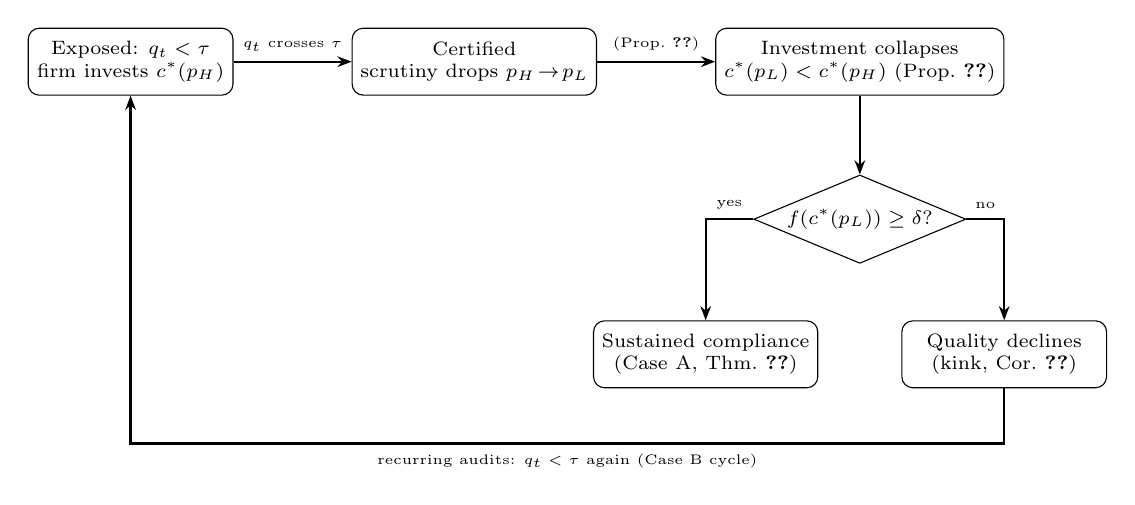
\begin{tikzpicture}[
  font=\scriptsize,
  box/.style={draw, rounded corners, align=center, minimum width=2.6cm, minimum height=0.85cm, inner sep=3pt},
  dec/.style={draw, diamond, align=center, aspect=2.4, inner sep=1pt},
  arr/.style={-{Stealth[length=1.8mm]}, thick},
  lbl/.style={font=\tiny, align=center}
]

\node[box] (n1) {Exposed: $q_t < \tau$\\ firm invests $c^*(p_H)$};
\node[box, right=1.5cm of n1] (n2) {Certified\\ scrutiny drops $p_H \!\to\! p_L$};
\node[box, right=1.5cm of n2] (n3) {Investment collapses\\ $c^*(p_L) < c^*(p_H)$ (Prop.~\ref{prop:drop})};
\node[dec, below=1.0cm of n3] (dec) {$f(c^*(p_L)) \geq \delta$?};
\node[box, below left=1.0cm and -0.15cm of dec] (n5a) {Sustained compliance\\ (Case A, Thm.~\ref{prop:recurring})};
\node[box, below right=1.0cm and -0.15cm of dec] (n5b) {Quality declines\\ (kink, Cor.~\ref{cor:kink})};

\draw[arr] (n1) -- node[lbl, above] {$q_t$ crosses $\tau$} (n2);
\draw[arr] (n2) -- node[lbl, above] {(Prop.~\ref{prop:drop})} (n3);
\draw[arr] (n3) -- (dec);
\draw[arr] (dec) -| node[lbl, pos=0.25, above] {yes} (n5a);
\draw[arr] (dec) -| node[lbl, pos=0.25, above] {no} (n5b);
\draw[arr] (n5b.south) -- ++(0,-0.7cm) -| node[lbl, pos=0.25, below] {recurring audits: $q_t < \tau$ again (Case B cycle)} ($(n1.south)+(0,-0.7cm)$) -- (n1.south);

\end{tikzpicture}
\caption{The mechanism, in outline: crossing $\tau$ triggers certification and a discrete investment drop (Proposition~\ref{prop:drop}); if growth still exceeds drift the firm sustains compliance, otherwise quality declines (Corollary~\ref{cor:kink}) and, under recurring audits, can fall back below $\tau$ and repeat (Theorem~\ref{prop:recurring}).}
\label{fig:pipeline}
\end{figure*}

We formalize this as a dynamic investment problem: a fairness-quality state drifts downward on its own unless the firm invests to counteract it, and the firm's only reason to invest is to reduce expected enforcement exposure, scaled by a scrutiny probability that drops discretely at first certification. A standard comparative-statics argument shows optimal investment is strictly increasing in perceived scrutiny, so investment drops discretely at certification (Proposition~\ref{prop:drop}), and under a condition on the safe-harbor discount relative to the drift rate, quality exhibits a \emph{kink}: rising while exposed, falling once shielded (Corollary~\ref{cor:kink}). Because real regimes recur rather than certifying once and for all, we generalize to lapsing certification (Section~\ref{sec:recurring}): the kink recurs indefinitely or the firm settles at a degraded steady state, both strictly worse long-run than no safe harbor at all (Theorem~\ref{prop:recurring}). Since firms plausibly differ in how strongly certification relieves scrutiny, a single common threshold sorts firms into these regimes by an unobserved characteristic (Section~\ref{sec:heterogeneous}), with an aggregate welfare cost we compute, and we take a first step toward the regulator's welfare-maximizing threshold (Section~\ref{sec:regulator}). The results are not an artifact of the specific functional forms used (Section~\ref{sec:sim-functionalform}), and replacing the perfectly-observed threshold with a noisily-observed one eliminates cycling once noise exceeds an analytically characterized threshold — below it, cycling persists, converging to the hard-threshold model's own behavior as noise vanishes (Section~\ref{sec:imperfectobs}).

The underlying mechanism — effort declining as monitoring probability declines — is not new; it organizes classical law-and-economics accounts of enforcement~\cite{becker1968crime,mookherjee1992monitoring}. Our contribution is formalizing it for point-in-time algorithmic certification and deriving the kink corollary as a testable consequence, which existing empirical critiques of audit regimes do not provide (Section~\ref{sec:related}).

\section{Related Work}
\label{sec:related}

\paragraph{Empirical critiques of algorithmic audit regimes.} A growing body of FAccT scholarship documents that existing algorithmic audit regimes fail to deliver the accountability they promise, largely through empirical and doctrinal analysis. Wright et al.~\cite{wright2024null} study 391 NYC employers' Local Law 144 compliance and introduce \emph{null compliance}: non-compliance that cannot be ascertained because the statute grants employers discretion over what is audited and disclosed. Groves et al.~\cite{groves2024auditing} similarly document structural weaknesses in the NYC regime's implementation. Neither formalizes a dynamic model or predicts investment changing systematically around certification. Power's account of auditing as institutional ``comfort rather than treatment''~\cite{power1997audit} is a qualitative diagnosis our model gives specific, falsifiable, dynamic form.

\paragraph{Enforcement economics.} That compliance investment responds to monitoring probability organizes the economics of law enforcement, from Becker's deterrence analysis~\cite{becker1968crime} through the inspection-game literature~\cite{mookherjee1992monitoring}. We adapt this to point-in-time algorithmic certification, where the discrete uncertified-to-certified transition is itself the event that changes perceived monitoring probability, deriving the kink corollary as a consequence of this structure.

\paragraph{Post-certification compliance relaxation elsewhere.} That passing an audit lowers subsequent compliance effort is documented, but not formalized dynamically, elsewhere. Kasper and Rablen~\cite{kasper2023tax} isolate a tax-compliance ``bomb-crater effect'': an audit lowering perceived re-audit probability causes compliance to fall, the closest empirical analogue to our mechanism. Gray and Mendeloff~\cite{gray2004declining} document OSHA inspections' injury-reducing effect attenuating from 19\% (1979--85) to statistically insignificant (1992--98). Both are empirical rather than formal.

\paragraph{Dynamic and repeated inspection.} Varas, Marinovic, and Skrzypacz~\cite{varas2020random} solve a continuous-time model where reputation depreciates between inspections and is re-earned, the closest scaffold for lapse-and-re-earn certification (Section~\ref{sec:recurring}). Che, Kim, and Mierendorff~\cite{che2024datadriven} extend this to a regulator learning compliance from noisy outcomes over time; Section~\ref{sec:imperfectobs} relaxes our own perfect-observation assumption more simply, finding cycling eliminated only once noise exceeds a threshold — a qualitative connection, where it holds, to their finding that imperfect information can sustain deterrence a fully-resolved state cannot. Fernandes and Phelan~\cite{fernandes2000recursive} and Halac and Prat~\cite{halac2016managerial} instead solve the fully forward-looking dynamic program against a proper continuation value; we adopt the myopic simplification for tractability (Section~\ref{sec:discussion}). Ball and Knoepfle~\cite{ball2023timing} show random inspection \emph{timing} outperforms predictable timing against decay — a lever distinct from our \emph{detection}-noise result, since our model normalizes cadence to one period.

\paragraph{Regulator-side mechanism design.} Macho-Stadler and P\'{e}rez-Castrillo~\cite{machostadler2006optimal} solve optimal emissions-audit allocation across strategically under-reporting firms; Huang and Zhu~\cite{huang2024zetar} give a Stackelberg information-design framework for privately-known types. Both treat non-compliance as static, without a decaying or lapse-and-re-earn state. None combines a certification event that shifts beliefs, a provable non-monotone effort trajectory, and a regulator anticipating it — what Section~\ref{sec:regulator} takes a first step toward, with the joint design problem under heterogeneity left open.

\paragraph{Algorithmic audit-gaming, institutional decoupling, and multiplicity.} Garcia Bourr\'{e}e et al.~\cite{garciabourree2025robust} and Basu and Das~\cite{basu2025fairgame} ask whether a \emph{fixed} audit can be certified manipulation-proof; our result is structurally different, since even a manipulation-proof, honestly-measured predicate can produce collapse through legitimate investment choices, not measurement gaming. Our claim that certification can decouple from the property it certifies echoes organizational sociology's ``myth and ceremony''~\cite{meyer1977institutionalized,edelman1992legal,bromley2012smoke}, which diagnoses decoupling generally where we contribute a specific formal mechanism. Model-multiplicity work~\cite{marx2020predictive,black2022model} shows a \emph{cross-sectional} indeterminacy in which model is certified, distinct from our \emph{temporal} claim about one model's quality evolving post-certification; De Toni et al.~\cite{detoni2025time} show individual recourse validity degrades under drift, a parallel temporal-invalidation result at the level of individual guarantees rather than firm-level incentives~\cite{lyons2021conceptualising}.

\section{Model}
\label{sec:model}

This section builds the model in stages: a firm's quality drifts down on its own and must be maintained by costly investment (below); the firm invests only to reduce its exposure to enforcement (Assumption~\ref{as:L}); and audits translate quality into a perceived probability of scrutiny that drops once the firm is certified (Equation~\ref{eq:pt}).

\paragraph{State and dynamics.} A firm operates an automated decision system with fairness-quality state $q_t \in \mathbb{R}$ at period $t$ (higher is fairer). Each period the firm chooses an investment $c_t \geq 0$ in maintaining or improving the system, and the state evolves as
\begin{equation}
q_{t+1} = q_t + f(c_t) - \delta,
\label{eq:dynamics}
\end{equation}
where $\delta > 0$ is a passive drift rate (e.g., from distribution shift) and $f$ converts investment into quality improvement.

\begin{assumption}
$f: \mathbb{R}_+ \to \mathbb{R}_+$ is twice continuously differentiable, strictly increasing, strictly concave with $f''(c)<0$ for every $c>0$ (stronger than strict concavity alone, satisfied by both $f(c)=a\sqrt{c}$ and $f(c)=ac^{1/3}$ below), $f(0)=0$, with Inada conditions $\lim_{c\to0^+}f'(c)=\infty$, $\lim_{c\to\infty}f'(c)=0$. This guarantees~\eqref{eq:foc} has a unique interior solution for every $p>0$ and reachable $q_{t+1}$.
\label{as:f}
\end{assumption}

\paragraph{Enforcement risk.} The firm's sole incentive to invest in $q$ is to reduce its expected exposure to litigation or regulatory enforcement, $L(q_t)$, decreasing in quality.

\begin{assumption}
$L: \mathbb{R} \to \mathbb{R}_+$ is twice continuously differentiable, strictly decreasing, strictly convex with $L''(q)>0$ for every $q$ (again stronger than strict convexity alone, satisfied by $L(q)=b/(q+1)$ and $L(q)=be^{-q}$ below). The calibration $L(q)=b/(q+1)$ requires $q>-1$, verified numerically along every simulated trajectory.
\label{as:L}
\end{assumption}

Let $p(t)$ denote the firm's perceived probability of scrutiny in period $t$. Audits occur periodically; once quality first reaches a legal threshold $\tau$ and the firm is certified, $p(t)$ drops discretely and stays low until the next scheduled audit:
\begin{equation}
p(t) =
\begin{cases}
p_H & \text{if exposed,} \\
p_L = \rho\, p_H, \ \rho \in (0,1) & \text{if certified,}
\end{cases}
\label{eq:pt}
\end{equation}
where \emph{exposed} means never certified or the most recent audit failed, and \emph{certified} means holding an unexpired safe harbor.

\begin{assumption}
The certification-triggered scrutiny discount satisfies $\rho \in (0,1)$ and is common knowledge to the firm.
\label{as:rho}
\end{assumption}

\paragraph{The firm's problem.} The firm chooses a sequence $\{c_t\}$ to minimize discounted expected cost,
\begin{equation}
\min_{\{c_t\}} \ \sum_{t} \beta^t \Big[ c_t + p(t)\, L(q_t) \Big], \qquad \beta \in (0,1).
\label{eq:objective}
\end{equation}
We solve this \emph{myopically}: each period the firm minimizes its own investment cost plus only the next period's expected litigation cost, approximating the exact Bellman condition $1+\beta V'(q_{t+1})f'(c_t)=0$ by replacing $V'(q_{t+1})$ with $p(t{+}1)L'(q_{t+1})$ — exact if $p(\cdot)$ is constant forever, and otherwise capturing the firm's immediate incentive while holding fixed its later behavior. Every result below holds at this scope; Section~\ref{sec:forwardlooking} checks two of Theorem~\ref{prop:recurring}'s three regimes against the fully forward-looking alternative.

The interior first-order condition at scrutiny level $p$ is
\begin{equation}
\beta\, p \cdot |L'(q_{t+1})| \cdot f'(c_t) = 1.
\label{eq:foc}
\end{equation}

\subsection{Discrete Investment Collapse}

\begin{proposition}
Under Assumptions~\ref{as:f}--\ref{as:rho}, the optimal investment $c^*(p)$ solving \eqref{eq:foc} is strictly increasing in $p$. Consequently, since $p(t)$ drops discretely from $p_H$ to $p_L = \rho\, p_H$ at first certification, optimal investment drops discretely: $c^*(p_L) < c^*(p_H)$. (The single-period objective $J(c;p)=c+\beta p\,L(q_t+f(c)-\delta)$ is strictly convex in $c$, giving a unique minimizer $c^*(p)$; the implicit function theorem applied to~\eqref{eq:foc} signs $dc^*/dp>0$. Full proof in Appendix~\ref{app:proofs}.)
\label{prop:drop}
\end{proposition}

\begin{lemma}[Joint monotonicity of optimal investment]
\label{lem:cstar}
Under Assumptions~\ref{as:f}--\ref{as:rho}, the optimal investment $c^*(q,p)$ solving~\eqref{eq:foc} at state $q$ and scrutiny $p>0$ is strictly increasing in $p$ holding $q$ fixed, and strictly decreasing in $q$ holding $p$ fixed, at every $(q,p)$. (The same convexity argument applies at every $(q,p)$; the cross-partials $\partial^2J/\partial c\,\partial p$ and $\partial^2J/\partial c\,\partial q$ have opposite signs, giving the opposite-signed comparative statics. Full proof in Appendix~\ref{app:proofs}.)
\end{lemma}

\begin{corollary}[Automatic non-overshoot]
\label{cor:slopebound}
Under Assumptions~\ref{as:f}--\ref{as:rho}, the one-period update map $h_p(q) \equiv q + f(c^*(q,p)) - \delta$ satisfies $h_p'(q) \in (0,1)$ at \emph{every} $q$ and $p>0$, for every $f,L$ satisfying Assumptions~\ref{as:f}--\ref{as:L}, with no bound on $f''$ or $L''$'s magnitude required. (Writing $h_p'(q)$ via Lemma~\ref{lem:cstar}'s two cross-partials, a common term cancels, leaving $h_p'(q)=L'f''/(L''f'^2+L'f'')$: numerator and denominator are both strictly positive, with the denominator strictly larger, so $h_p'(q)\in(0,1)$; full proof in Appendix~\ref{app:proofs}.)
\end{corollary}

Proposition~\ref{prop:drop} shows investment falls at certification; whether this is consequential for $q_t$'s trajectory depends on how the new investment compares to $\delta$.

\begin{corollary}
If $f(c^*(\tau,p_L)) < \delta \leq f(c^*(\tau,p_H))$ — evaluated at the certification date $q_t=\tau$ — so pre-certification investment offset drift while post-certification investment does not, then $q_t$ is non-decreasing just before first certification and strictly decreasing just after: a kink at the certification date. This holds whenever $\rho$ is strong enough to pull $f(c^*(p_L))$ below $\delta$ without $f(c^*(p_H))$ also falling below it (Proposition~\ref{prop:drop}) — equivalently (Lemma~\ref{lem:cstar}), exactly $q^*(p_L) < \tau \leq q^*(p_H)$, the same region driving Theorem~\ref{prop:recurring}'s cycling case.
\label{cor:kink}
\end{corollary}

\subsection{Recurring Audits and Lapsing Certification}
\label{sec:recurring}

Corollary~\ref{cor:kink} describes a firm's \emph{first} certification, treating the safe harbor as permanent. Real audit regimes re-evaluate periodically (NYC Local Law 144~\cite{nyc2021ll144} requires an annual bias audit), so certification can lapse. We generalize \eqref{eq:pt} to a state-contingent rule, normalizing the audit cadence to one model period:
\begin{equation}
p(t) = p_H \cdot \mathbf{1}\{q_t < \tau\} + p_L \cdot \mathbf{1}\{q_t \geq \tau\},
\label{eq:pt-recurring}
\end{equation}
so certification is granted exactly when quality meets $\tau$ and lapses immediately once it falls below — a strict generalization of \eqref{eq:pt}'s one-time, permanent switch.

\begin{assumption}
\label{as:steadystate}
There exists $c_\delta \geq 0$ with $f(c_\delta) = \delta$, and for every $p > 0$ a unique $q^*(p)$ solving
\begin{equation}
\beta\, p\, |L'(q^*(p))|\, f'(c_\delta) = 1,
\label{eq:steadystate}
\end{equation}
by $|L'|$ continuous, strictly decreasing, with full range on the relevant interval.
\end{assumption}

$q^*(p)$ is the quality level at which investing exactly enough to offset drift is myopically optimal under constant scrutiny $p$: a \emph{steady state} of \eqref{eq:dynamics} the firm has no incentive to move away from.

\begin{proposition}
Under Assumptions~\ref{as:f}--\ref{as:steadystate}, $q^*(p)$ is strictly increasing in $p$. (From~\eqref{eq:steadystate}, $|L'(q^*(p))|=1/(\beta p f'(c_\delta))$ is strictly decreasing in $p$ on the right, so the unique solution rises with $p$ since $|L'|$ is strictly decreasing in $q$.)
\label{prop:steadystate}
\end{proposition}

\begin{corollary}[Comparative statics in the drift rate]
\label{cor:deltacompstat}
Writing $q^*(p,\delta)$ to make the dependence on $\delta$ explicit: under Assumptions~\ref{as:f}--\ref{as:steadystate}, $q^*(p,\delta)$ is strictly decreasing in $\delta$ for fixed $p$. (Since $c_\delta\equiv f^{-1}(\delta)$ rises with $\delta$ and $f'$ is decreasing, $f'(c_\delta)$ falls as $\delta$ rises, pushing~\eqref{eq:steadystate}'s right-hand side up and so $q^*(p,\delta)$ down: a firm facing more drift settles, all else equal, at lower steady-state quality.)
\end{corollary}

\begin{mainthm}[Recurring audits]
Under Assumptions~\ref{as:f}--\ref{as:steadystate} and the state-contingent rule~\eqref{eq:pt-recurring}, exactly one of three regimes occurs:
\begin{enumerate}
\item[(a)] \textbf{Sustained certification.} If $\tau \leq q^*(p_L)$, the trajectory converges to the stable steady state $q^*(p_L) \geq \tau$, and the firm remains certified indefinitely.
\item[(b)] \textbf{Perpetual cycling.} If $q^*(p_L) < \tau < q^*(p_H)$, no steady state is compatible with the threshold: the firm climbs toward $q^*(p_H)$ while exposed, is certified once $q_t \geq \tau$, declines while shielded, and reverts to exposed once $q_t$ falls back below $\tau$, repeating indefinitely. The trajectory is eventually confined to a bounded interval it crosses infinitely often; we call this pattern \emph{cycling}. (The proof establishes this boundedness, infinite recurrence, and the long-run average bounds below, but not that the orbit is eventually exactly periodic — see Appendix~\ref{app:proofs}.)
\item[(c)] \textbf{Perpetual exclusion.} If $\tau \geq q^*(p_H)$, the trajectory converges to $q^*(p_H) \leq \tau$ under permanent exposure, and the firm is never certified. (The boundary $\tau=q^*(p_H)$ belongs here, not to Case (b): monotone convergence approaches but never attains $q^*(p_H)$ in finite time.)
\end{enumerate}
In all three regimes, long-run (time-averaged, in case (b)) quality is bounded above by $q^*(p_H)$; strictly below it whenever $\rho<1$ in cases (a) and (b), equal to it in case (c). Recurring certification under any positive safe-harbor discount thus produces strictly worse long-run outcomes than a no-safe-harbor counterfactual whenever certification is ever achieved, even though the firm never permanently fails an audit.
\label{prop:recurring}
\end{mainthm}

\begin{proof}[Proof sketch]
Corollary~\ref{cor:slopebound} makes $h_p$ strictly increasing everywhere with $h_p(q^*(p))=q^*(p)$, so $h_p(q)$ lies strictly between $q$ and $q^*(p)$ on either side (no overshoot). In Case (a), a firm below $\tau$ rises toward $q^*(p_H)>\tau$ exposed, and once certified stays at or above $\tau$ forever, converging to $q^*(p_L)$; Case (c) is symmetric. In Case (b), the same property makes $[h_{p_L}(\tau),h_{p_H}(\tau))$ forward-invariant and eventually entered — resting on either side would contradict that side's own steady state — giving the average bound without exact periodicity (a stronger claim not established; Appendix~\ref{app:proofs} explains why).
\end{proof}

Case (b) generalizes Corollary~\ref{cor:kink} to an indefinitely repeating sequence of kinks; Case (c) is a boundary case for completeness.

\subsection{Robustness to Forward-Looking Optimization}
\label{sec:forwardlooking}

A fully rational, forward-looking firm internalizes that today's investment lowers litigation exposure in \emph{every} future period, not only the next, and so might invest more, potentially blunting the collapse. In the two regimes where scrutiny is eventually constant forever — Cases (a) and (c) — this does not overturn the finding: the rational firm's steady state is the myopic formula evaluated at an inflated effective scrutiny level.

\begin{proposition}[Forward-looking steady state under constant scrutiny]
\label{prop:forwardlooking}
Suppose scrutiny is held at a constant $p>0$ forever — as it eventually is along the \emph{myopic} firm's path in Cases (a) and (c) — and let $V$ solve \eqref{eq:objective} exactly. (It is not established that a \emph{forward-looking} firm's own path also settles into constant $p$; this characterizes what such a steady state would look like, if reached.) If the exact problem admits a steady state $q^{\dagger}(p)$ at which the firm invests $c_\delta$ forever, then
\[
q^{\dagger}(p) = q^*\!\left(\frac{p}{1-\beta}\right),
\]
so $q^{\dagger}(p)$ is strictly increasing in $p$ and $q^{\dagger}(p) > q^*(p)$ for every $p>0,\beta\in(0,1)$: forward-looking optimization preserves the comparative static driving Theorem~\ref{prop:recurring} while raising sustained quality. (The envelope-theorem recursion for $V'$ becomes stationary at such a steady state, reproducing~\eqref{eq:steadystate} with $p$ replaced by $p/(1-\beta)>p$. Full proof in Appendix~\ref{app:proofs}.)
\end{proposition}

This is conditional on such a steady state existing (left open, as is Assumption~\ref{as:steadystate} for the myopic model) and does not extend to Case (b), where scrutiny is never constant along the equilibrium path; whether forward-looking cycling shrinks, grows, or disappears needs numerical dynamic programming (Section~\ref{sec:discussion}).

\subsection{Heterogeneous Firms}
\label{sec:heterogeneous}

Theorem~\ref{prop:recurring} treats $\rho$ as common across firms, but its strength plausibly varies with unobserved characteristics (litigation exposure, visibility, unionization).

\begin{proposition}[Firm sorting under a common threshold]
Suppose firms differ in $\rho_i \in (0,1)$ but share $p_H$ and $\tau < q^*(p_H)$. Since $q^*(\rho p_H)$ is strictly increasing in $\rho$ (Proposition~\ref{prop:steadystate}), there is at most one cutoff $\rho_A(\tau)$ solving $q^*(\rho_A(\tau) p_H) = \tau$, existing in $(0,1)$ provided $\tau > \lim_{\rho\to0^+}q^*(\rho p_H)$ (holds at our calibration: this limit is $-1<\tau=0.80$). Firm $i$ falls into Case (a) if $\rho_i \geq \rho_A(\tau)$, Case (b) otherwise (immediate from Theorem~\ref{prop:recurring}'s case conditions).
\label{prop:heterogeneous}
\end{proposition}

\begin{remark}[Heterogeneous exposure and drift]
\label{rem:heterogeneous-general}
The proof applies verbatim if firms instead differ in baseline exposure $p_{H,i}$ or drift $\delta_i$ (Corollary~\ref{cor:deltacompstat}), sorting on $p_{L,i}\equiv\rho_i p_{H,i}$: Case (a) if $q^*(p_{L,i},\delta_i)\geq\tau$, Case (c) if $\tau\geq q^*(p_{H,i},\delta_i)$, Case (b) otherwise. Sorting risk is governed by $p_{L,i}$, not $\rho_i$ alone. Corollary~\ref{cor:aggwelfare}'s integral extends the same way, with a third term for Case (c).
\end{remark}

A single audit rule thus sorts firms into starkly different regimes: weak-safe-harbor firms ($\rho_i$ near $1$) settle into stable, degraded compliance; strong-safe-harbor firms cycle perpetually. Pass/fail records cannot distinguish Case (a)'s degraded-but-stable compliance from genuine compliance, and Case (b)'s cycling surfaces without flagging \emph{why}, or that both underperform the no-safe-harbor benchmark. At our calibration, $\rho_A(\tau)=0.5015$, confirmed numerically (Figure~\ref{fig:rhosweep}).

\begin{corollary}[Aggregate welfare loss]
\label{cor:aggwelfare}
Let firms be drawn from $\rho_i\sim G$ on $(0,1)$, sharing $p_H$, $\tau<q^*(p_H)$. For a Case (b) firm, write $\bar q_B(\tau,\rho)$ for the $\limsup$ time-average bounded in Theorem~\ref{prop:recurring}'s proof. Aggregate welfare is
\begin{equation}
W_{\mathrm{agg}}(\tau, G) = \int_0^{\rho_A(\tau)} \bar{q}_B(\tau,\rho)\, dG(\rho) \;+\; \int_{\rho_A(\tau)}^{1} q^*(\rho\, p_H)\, dG(\rho),
\label{eq:aggwelfare}
\end{equation}
cycling firms then sustained firms. The welfare loss $q^*(p_H) - W_{\mathrm{agg}}(\tau, G)$ is strictly positive for every $G$ on $(0,1)$, since $q^*(\rho p_H) < q^*(p_H)$ even in Case (a) (Proposition~\ref{prop:steadystate}), and cycling firms lose further still.
\end{corollary}

Section~\ref{sec:sim-heterogeneous} computes this under two illustrative distributions.

\subsection{Imperfect Observation}
\label{sec:imperfectobs}

Sections~\ref{sec:recurring}--\ref{sec:heterogeneous} assume audits perfectly reveal whether $q_t \geq \tau$; real audits are noisy proxies, so we replace the hard threshold~\eqref{eq:pt-recurring} with a smooth detection probability $\pi: \mathbb{R} \to (0,1)$, strictly increasing with $\pi(-\infty)=0$, $\pi(\infty)=1$ — e.g.\ the logistic $\pi(q) = 1/(1+\exp(-(q-\tau)/\sigma))$ — and redefine
\begin{equation}
p(q) = p_H - \pi(q)\,(p_H - p_L),
\label{eq:pt-noisy}
\end{equation}
so certification is probabilistic, with $\pi(q)$ the probability of being certified at $q$. As $\sigma \to 0$, $\pi(q) \to \mathbf{1}\{q \geq \tau\}$ and~\eqref{eq:pt-noisy} recovers~\eqref{eq:pt-recurring} exactly.

\begin{assumption}
$\pi$ is continuous and strictly increasing with $\pi(-\infty)=0$, $\pi(\infty)=1$.
\label{as:noisy}
\end{assumption}

\begin{proposition}[Imperfect observation: a unique crossing point, not always stable]
Under Assumptions~\ref{as:f}--\ref{as:noisy}, for every $\sigma > 0$ the dynamics under~\eqref{eq:pt-noisy} have a unique steady state $q^{**}(\sigma) \in (q^*(p_L), q^*(p_H))$, unconditionally — no kink condition needed. If in addition $f(c^*(p_H)) - \delta > 0 > f(c^*(p_L)) - \delta$ (the kink condition, equivalently $q^*(p_L)<\tau<q^*(p_H)$), then $q^{**}(\sigma) \to \tau$ as $\sigma \to 0$.

This steady state is \emph{not}, however, stable for every $\sigma>0$: under the logistic $\pi$ and the kink condition, there is a $\sigma_0>0$ such that for $\sigma<\sigma_0$, $q^{**}(\sigma)$ is \emph{repelling}, so cycling is eliminated only once $\sigma$ exceeds $\sigma_0$. Below it (Section~\ref{sec:sim-imperfectobs}), the trajectory settles into a bounded oscillation whose amplitude grows, and whose time-average approaches the hard-threshold cycling mean, as $\sigma\to0$.
\label{prop:imperfectobs}
\end{proposition}

\begin{proof}[Proof sketch]
Since $p(q)\in(p_L,p_H)$ strictly for every finite $q$, bounding $c^*(q,p(q))$ between $c^*(q,p_L)$ and $c^*(q,p_H)$ shows $g(q)\equiv f(c^*(q,p(q)))-\delta$ is positive for $q\le q^*(p_L)$ and negative for $q\ge q^*(p_H)$ unconditionally, giving existence and uniqueness with no kink condition needed; $q^{**}(\sigma)\to\tau$ under the kink condition follows from the same bound at a fixed $q$ as $\sigma\to0$. Instability for small $\sigma$ comes from the fixed-point slope $k'(q^{**}(\sigma))$: a bounded term (Corollary~\ref{cor:slopebound}'s bound) minus a term that, for the logistic $\pi$, grows like $1/\sigma$, so $k'(q^{**}(\sigma))\to-\infty$ as $\sigma\to0$. Full proof in Appendix~\ref{app:proofs}.
\end{proof}

Section~\ref{sec:discussion} discusses the mechanism and its policy implications; Section~\ref{sec:sim-imperfectobs} confirms both regimes numerically.

\section{Illustrative Simulation}
\label{sec:sim}

Code and data to reproduce all simulations and figures in this paper are available at \url{https://anonymous.4open.science/r/cert_fore/}.

To confirm the kink condition (Corollary~\ref{cor:kink}) is not vacuous, we simulate the model under $f(c) = a\sqrt{c}$, $L(q) = b/(q+1)$, with $a = 0.30$, $b = 6.80$, $\beta = 0.95$, $\delta = 0.045$, $\tau = 0.80$, $p_H = 1.0$, $\rho = 0.30$ — chosen for tractability, not because the mechanism depends on them (Section~\ref{sec:sim-functionalform} confirms a structurally unrelated pair).

At $q=\tau$, $c^*(p_H)=0.0818$ and $c^*(p_L)=0.0084$, giving $f(c^*(p_H))=0.0858$ and $f(c^*(p_L))=0.0275$: the kink condition $f(c^*(p_L))<\delta\leq f(c^*(p_H))$ holds. Figure~\ref{fig:qc}(a) plots the resulting $q_t$ against a no-discount ablation ($p$ held at $p_H$ throughout). Starting from $q_0=0.30$, both trajectories climb identically while exposed; the foreclosure trajectory is first certified at $t=8$, peaks at $q=0.825$, and declines to $q=0.481$ by $t=39$ despite never failing a subsequent audit, while the ablation continues to $q=1.348$. Figure~\ref{fig:qc}(b) shows investment falling by an order of magnitude ($0.085\to0.008$) in the single period spanning certification, with no recovery.

\begin{figure}[t]
\centering
\begin{minipage}{0.49\linewidth}
\centering
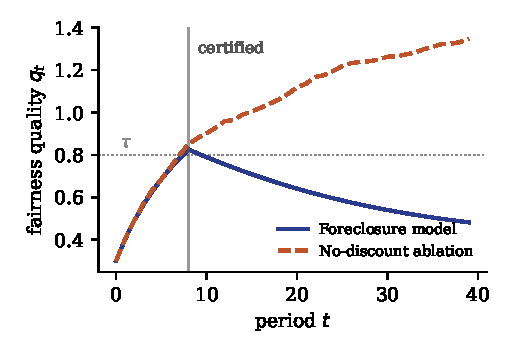
\includegraphics[width=\linewidth]{figures/fig_q.pdf}
\\ (a) Fairness quality $q_t$
\end{minipage}
\hfill
\begin{minipage}{0.49\linewidth}
\centering
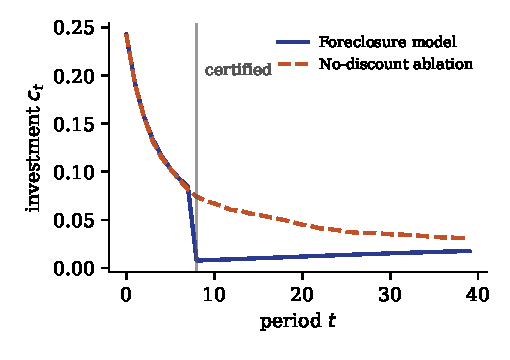
\includegraphics[width=\linewidth]{figures/fig_c.pdf}
\\ (b) Investment $c_t$
\end{minipage}
\caption{(a) The foreclosure model's quality trajectory peaks exactly at certification ($t=8$) and declines, while the no-discount ablation keeps improving under constant scrutiny. (b) Investment falls roughly tenfold in the single period spanning certification, with no recovery.}
\label{fig:qc}
\end{figure}

\subsection{Recurring Audits: Simulating Both Cases}
\label{sec:sim-recurring}

We verify Theorem~\ref{prop:recurring} on the same parameterization, using the closed form $q^*(p) = \sqrt{p\,\beta\,a^2 b / (2\delta)} - 1$ (Appendix~\ref{app:derivation}): $q^*(p_H)=1.542$. At $\rho=0.30$ ($q^*(p_L)=0.392<\tau<q^*(p_H)$: Case B), simulating~\eqref{eq:pt-recurring} for 120 periods produces sustained cycling: over $t\geq60$, $q_t$ oscillates between $0.783$ and $0.840$ with a period of 3--4 audit cycles, time-average $0.813$, strictly below $q^*(p_H)$. At $\rho=0.60$ ($\tau\leq q^*(p_L)=0.969$: Case A), the firm converges to a stable, permanently certified steady state near $q^*(p_L)$ — still strictly below $q^*(p_H)$, so the welfare loss persists even without cycling. Figure~\ref{fig:recurring} plots both.

\begin{figure}[t]
\centering
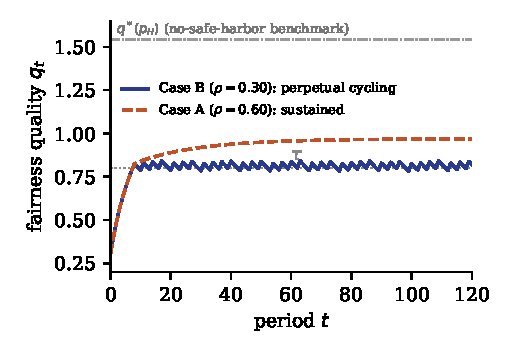
\includegraphics[width=0.55\linewidth]{figures/fig_recurring.pdf}
\caption{Recurring audits: at $\rho=0.30$ (Case B) the firm cycles indefinitely across $\tau$; at $\rho=0.60$ (Case A) it settles into permanent certification, below $q^*(p_H)$ in both cases.}
\label{fig:recurring}
\end{figure}

\subsection{Robustness Checks}
\label{sec:sim-robustness}

Four robustness checks; the $\rho$-sweep's extra figure and detail, and the real-disclosures calibration's full detail, are in Appendix~\ref{app:extra-sim}.

\paragraph{Safe-harbor discount.} Sweeping $\rho\in(0.05,0.95)$ at $\tau=0.80$ (Figure~\ref{fig:rhosweep}) confirms the Case A/B split is not a knife-edge artifact: the boundary falls at $\rho_A(\tau)=0.5015$, matching Proposition~\ref{prop:heterogeneous}'s cutoff to four decimals, with time-averaged quality in the cycling region staying flat in $[0.804,0.817]$ across a tenfold range of $\rho$ — once cycling, the outcome is insensitive to exactly how strong the discount is, only to whether it is strong enough to place the firm there. (This sweep also supplies the data behind Sections~\ref{sec:heterogeneous} and~\ref{sec:regulator}.) Separately sweeping $\beta\in[0.80,0.99]$ and $\delta\in[0.010,0.090]$ confirms cycling is robust to $\beta$ and that $\delta$ moves the firm through all three regimes, consistent with Corollary~\ref{cor:deltacompstat}.

\begin{figure}[t]
\centering
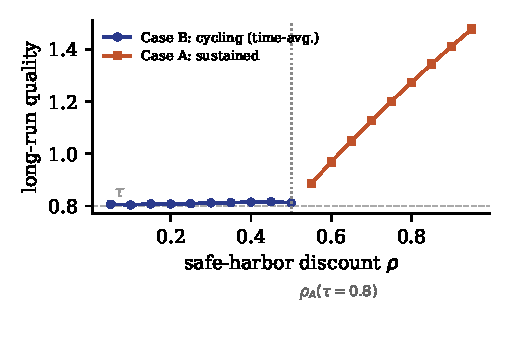
\includegraphics[width=0.55\linewidth]{figures/fig_rhosweep.pdf}
\caption{Long-run quality as $\rho$ varies, $\tau=0.80$ fixed. The Case A/B boundary at $\rho_A=0.5015$ matches the closed-form prediction; within Case B, the time-average is roughly flat across a wide range of $\rho$.}
\label{fig:rhosweep}
\end{figure}

\paragraph{Functional form.}\label{sec:sim-functionalform} The results above use $f(c)=a\sqrt{c}$, $L(q)=b/(q+1)$. To check this is not load-bearing, we repeat the four central checks under a structurally different pair, $f(c)=ac^{1/3}$ and $L(q)=be^{-q}$ ($a=0.55$, $b=3.20$), recalibrating $\tau=3.80$ to sit between this pair's own steady states ($q^*(p_L)=3.218$, $q^*(p_H)=4.422$ at $\rho=0.30$) rather than reuse the original calibration's scale. Table~\ref{tab:functionalform} shows all four reproduce. (One subtlety: $c^*(p)$ and $\delta$ are not directly commensurate, so the kink condition is stated via $f(c^*(p))$ rather than $c^*(p)$ itself — the two comparisons coincide numerically under $\sqrt{c}$ because $f$ is near-linear there, but diverge visibly here.)

\begin{table}[t]
\centering
\footnotesize
\caption{Central results reproduced under $f(c)=a\,c^{1/3}$, $L(q)=b\,e^{-q}$ ($a=0.55$, $b=3.20$, $\tau=3.80$, $\rho=0.30$).}
\label{tab:functionalform}
\begin{tabular}{@{}p{0.32\linewidth}p{0.6\linewidth}@{}}
\toprule
Check & Result \\
\midrule
Discrete investment collapse & $c^*(p_L)=0.0002 < c^*(p_H)=0.0014$ \\[2pt]
Kink condition & $f(c^*(p_L))=0.034 < \delta=0.045 \leq f(c^*(p_H))=0.061$ \\[2pt]
Single-certification kink & peaks at $t{=}55$ ($q{=}3.815$), declines to $q{=}3.221$ by $t{=}300$ \\[2pt]
Recurring-audit cycling & $123$ regime switches in tail; mean $3.803 < q^*(p_H){=}4.422$ \\
\bottomrule
\end{tabular}
\end{table}

\paragraph{Firm heterogeneity.}\label{sec:sim-heterogeneous} Evaluating Corollary~\ref{cor:aggwelfare} under $\rho_i\sim\mathrm{Uniform}(0.05,0.95)$ gives aggregate welfare $0.983$, a $36.2\%$ loss relative to $q^*(p_H)$ with $50.2\%$ of firms cycling; under $\rho_i\sim\mathrm{Beta}(4,2)$ (weighted toward weak safe-harbor effects, a conservative stand-in for a population where severe effects are the exception), loss falls to $30.4\%$ with $18.9\%$ cycling but does not disappear — even Case (a) firms sustain quality strictly below $q^*(p_H)$ whenever $\rho_i<1$ (Table~\ref{tab:aggwelfare}).

\begin{table}[t]
\centering
\caption{Aggregate welfare loss under two firm-population distributions, $\tau=0.80$, $q^*(p_H)=1.542$.}
\label{tab:aggwelfare}
\begin{tabular}{@{}lccc@{}}
\toprule
Distribution of $\rho_i$ & $W_{\mathrm{agg}}$ & Loss (\% of $q^*(p_H)$) & \% cycling \\
\midrule
Uniform$(0.05,0.95)$ & $0.983$ & $36.2\%$ & $50.2\%$ \\
Beta$(4,2)$, rescaled & $1.072$ & $30.4\%$ & $18.9\%$ \\
\bottomrule
\end{tabular}
\end{table}

\paragraph{Calibrating to real audit disclosures.}\label{sec:calibration} NYC Local Law 144 disclosure data grounds $\tau=0.80$ empirically. Wright et al.~\cite{wright2024null} found 96\% of 386 impact-ratio measurements (late 2023) exceeded $0.8$; Gerchick et al.~\cite{gerchick2025auditing}, through November 2024, found a larger below-threshold share (23--28\% of group-level results) — a discrepancy we attribute to sampling and methodology differences rather than resolve. The latter is inconsistent with a population of only Case A firms (which, once certified, stay at or above $\tau$) and more consistent with Case B firms cycling around it, though we stop short of testing the dynamic predictions directly: only 13 same-employer report-pairs are documented, with overwritten disclosures and no tool-version identifiers (Appendix~\ref{app:extra-sim}, Section~\ref{sec:discussion}).

\subsection{Imperfect Observation}
\label{sec:sim-imperfectobs}

We verify Proposition~\ref{prop:imperfectobs} using the logistic $\pi(q)=1/(1+\exp(-(q-\tau)/\sigma))$, with investment evaluated against scrutiny at the firm's \emph{current} state $p(q_t)$, exactly as specified.\footnote{An earlier version instead evaluated scrutiny at the post-investment state and added a term not implied by the proposition; it is kept in the replication code for reference only and is not the source of the numbers here.} The unique fixed point $q^{**}(\sigma)$ matches the closed-form prediction, converging to $\tau=0.800$ as $\sigma\to0$ for every $\sigma$ down to $10^{-5}$. The simulated \emph{trajectory}, however, only converges above $\sigma_0\approx0.0063$ (where the fixed point's slope crosses $-1$); below it, it settles into persistent bounded oscillation instead (Figure~\ref{fig:imperfectobs}). Just above threshold, $q^{**}(0.01)=0.809$; at $\sigma=1.0$, $q^{**}=0.995$, below $q^*(p_H)=1.542$ but well above $\tau$ and the hard-threshold cycling mean $0.8125$. Below threshold, amplitude widens as $\sigma\to0$ and the time-average converges to $0.812$, matching that cycling mean to three decimals.

\begin{figure}[t]
\centering
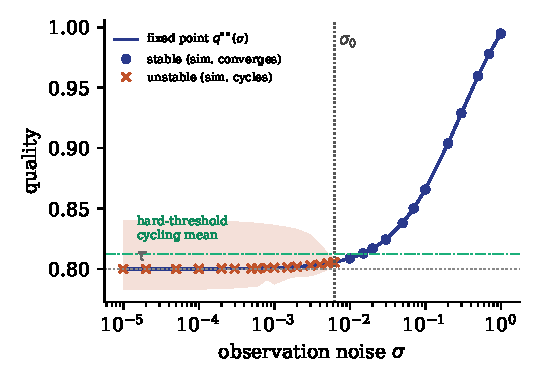
\includegraphics[width=0.55\linewidth]{figures/fig_imperfectobs.pdf}
\caption{Quality under imperfect observation as detection noise $\sigma$ varies (log scale). The fixed point $q^{**}(\sigma)$ converges to $\tau$ as $\sigma\to0$ regardless of stability; circles mark simulated convergence, crosses mark cycling (shaded: tail range) below $\sigma_0$.}
\label{fig:imperfectobs}
\end{figure}

Above $\sigma_0$, higher noise raising quality is the opposite of the naive ``noisier audits are worse'' intuition; Section~\ref{sec:imperfectobs} explains why this does not generalize to noise that is merely uninformative rather than cliff-edge-removing.

\section{The Regulator's Design Problem}
\label{sec:regulator}

The preceding sections characterize a firm's response to a given audit design. We now ask what threshold a regulator should choose, anticipating that response, treating $p_H$, $\rho$, $\delta$, $f$, $L$ as exogenous features of the audited population. Suppose the regulator's objective is long-run quality, $W(\tau)$, defined by Theorem~\ref{prop:recurring}'s three cases:
\begin{equation}
W(\tau) =
\begin{cases}
q^*(p_L) & \tau \leq q^*(p_L) \quad \text{[Case (a)]} \\
\bar{q}_B(\tau) & q^*(p_L) < \tau < q^*(p_H) \quad \text{[Case (b)]} \\
q^*(p_H) & \tau \geq q^*(p_H) \quad \text{[Case (c)]}
\end{cases}
\label{eq:regulatorobjective}
\end{equation}
where $\bar{q}_B(\tau)$ is $\bar{q}_B(\tau,\rho)$ from Corollary~\ref{cor:aggwelfare} with $\rho=0.30$ fixed throughout this section.

\begin{proposition}[Boundary regions are flat]
$W(\tau) = q^*(p_L)$ for every $\tau \leq q^*(p_L)$, and $W(\tau) = q^*(p_H)$ for every $\tau \geq q^*(p_H)$. (Immediate from Theorem~\ref{prop:recurring}: in Case (a), long-run quality is $q^*(p_L)$ regardless of the specific $\tau$; in Case (c), it is $q^*(p_H)$ regardless of the specific $\tau$, since the firm converges there without ever reaching $\tau$, including at $\tau=q^*(p_H)$ itself.)
\label{prop:flatregions}
\end{proposition}

So the design question lives entirely in Case (b), where we lack a general proof that $\bar{q}_B(\tau)$ is monotonic. Sweeping $\tau$ across $(0.30,1.55)$ at $\rho=0.30$ (Figure~\ref{fig:tausweep}), $\bar{q}_B(\tau)$ increases at every sampled point, from $W=0.427$ at $\tau=0.40$ to $W=1.487$ at $\tau=1.50$, just below $q^*(p_H)=1.542$, with no reversal. Combined with Proposition~\ref{prop:flatregions}, welfare is non-decreasing across the entire range, attaining its maximum $q^*(p_H)$ at $\tau^\star=q^*(p_H)$ and beyond — a numerically-supported trend, not a proven limit.

This maximum is degenerate: at $\tau\geq q^*(p_H)$ certification is never granted (Case (c)), so ``$\tau^\star=q^*(p_H)$'' is indistinguishable from eliminating the safe harbor outright, not a design recommendation — and not because the firm invests nothing there, since it still invests $c_\delta>0$ forever (Appendix~\ref{app:extra-sim} checks this against a cost-adjusted objective and finds the recommendation robust). The substantive content is that welfare rises monotonically through the achievable Case (b) range, approaching but never exceeding $q^*(p_H)$: a regulator wanting the safe harbor to remain operative should target $\tau$ close to, but strictly below, $q^*(p_H)$. Since $q^*(p_H)$ depends only on cost structure and drift, not $\rho$, it can be estimated from firm behavior under negligible safe-harbor effects (e.g., early in an enforcement regime) — a concrete target distinct from calibrating $\tau$ to a population-wide norm, closer to how the four-fifths rule was historically set.

\begin{figure}[t]
\centering
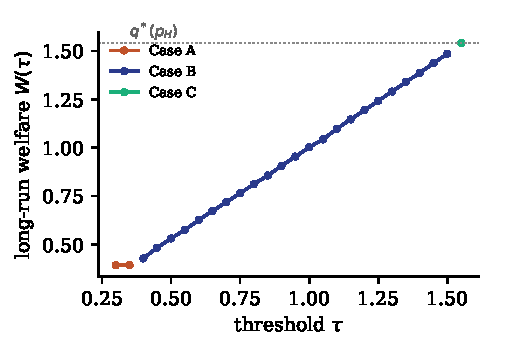
\includegraphics[width=0.55\linewidth]{figures/fig_tausweep.pdf}
\caption{Long-run welfare $W(\tau)$ as the threshold varies, $\rho=0.30$ fixed. Flat below $q^*(p_L)$ and at or above $q^*(p_H)$ (Proposition~\ref{prop:flatregions}, proven); numerically monotonic in between (Case B), approaching $q^*(p_H)$ at the upper boundary.}
\label{fig:tausweep}
\end{figure}

\section{Discussion}
\label{sec:discussion}

\paragraph{Implications for audit design.} Audit design faces a failure mode distinct from threshold miscalibration: a well-calibrated threshold can still produce worse long-run outcomes than no safe harbor at all, if certification confers a sufficiently strong one, structurally rather than as a one-time artifact (Theorem~\ref{prop:recurring}). Case (a)'s degraded steady state is invisible from pass/fail records, since such a firm never subsequently fails; Case (b)'s cycling surfaces as repeated failing and re-passing, but nothing flags why. Both underperform the no-safe-harbor counterfactual, and Section~\ref{sec:sim-heterogeneous} puts a number on it: roughly a third of achievable quality under a stylized population. One lever independent of the threshold: raising $\rho$ toward $1$ (e.g., preserving contestability rights after certification). A second, more speculative lever — shortening the audit interval relative to drift — is suggestive but not evaluable here, since our model normalizes cadence to a single period; Ball and Knoepfle~\cite{ball2023timing} give the closer formal treatment.

\paragraph{Imperfect observation is a third lever, with a caveat.} Proposition~\ref{prop:imperfectobs} adds a lever the first two do not suggest: a noisily-observed threshold gives a single crossing point in place of two discrete levels, and above threshold $\sigma_0$ this point is stable and, in our simulations, raises quality — against the usual presumption that noisier audits are worse. But below $\sigma_0$ the point is unstable and cycling persists instead, converging to the hard-threshold model's behavior as noise vanishes. What matters is not imprecision per se but removing the cliff edge a firm can fully escape past; whether that stabilizes or destabilizes depends on how fast scrutiny changes near the crossing point, which is why the benefit reverses at small $\sigma$. A noisy audit that is also biased or gameable is not covered. We read this as a reason to distinguish cliff-edge-removing noise from noise that merely degrades information, not a recommendation to make audits noisier on purpose.

\paragraph{The regulator's design problem, and what remains open.} Welfare is non-decreasing in $\tau$ up to $q^*(p_H)$ and flat thereafter, but $\tau=q^*(p_H)$ attains that maximum only by making certification unattainable, so the recommendation is $\tau$ close to, but strictly below it — a numerically-supported conjecture, holding $\rho$ fixed (Section~\ref{sec:regulator}). This falls short of the fully strategic problem: jointly choosing $\tau$ and a policy shaping $\rho$ under heterogeneity (Section~\ref{sec:heterogeneous}) rather than a representative firm. Section~\ref{sec:related}'s mechanism-design literature~\cite{machostadler2006optimal,huang2024zetar,varas2020random} gives relevant machinery for a related but distinct problem; combining it with our results under heterogeneity is the natural next extension.

\paragraph{Limitations.} This is primarily theoretical: Sections~\ref{sec:sim}--\ref{sec:sim-functionalform} show the central results are satisfiable and not an artifact of functional form, but the imperfect-observation and heterogeneity results are checked only at our calibration. Section~\ref{sec:calibration} anchors $\tau=0.80$ against real disclosure statistics but cannot test the dynamic predictions directly, since the needed firm-level panel does not yet exist. The logistic detection function is a modeling convenience, and the noise-raises-quality finding holds only above $\sigma_0$, established numerically. Section~\ref{sec:regulator}'s result likewise holds $\rho$ fixed, with a single representative firm.

\section{Conclusion}

We have shown that a passing algorithmic audit can be the proximate cause of a system's subsequent decline: certification's effect on a firm's own investment incentives, distinct from measurement error or threshold miscalibration. Under recurring audits this is a structural choice between a permanently degraded steady state and perpetual cycling, both strictly worse long-run than no safe harbor at all. The degraded steady state is invisible to a regulator observing only pass/fail records, since such a firm never subsequently fails; cycling surfaces as a repeated fail-then-pass pattern, but nothing flags why. The mechanism survives firm heterogeneity and a different functional-form pair; cycling turns out, unexpectedly, to disappear once the threshold is observed imperfectly — but only once noise exceeds an identified threshold, below which it persists and converges to the hard-threshold model's behavior. These predictions are falsifiable, giving regulators a concrete additional design target: safe-harbor strength, audit precision, and threshold choice together.

\paragraph{Limitations.} The results are primarily theoretical: functional forms and parameters are chosen for tractability, not fit to a deployed regime, and Section~\ref{sec:calibration} anchors the threshold against real disclosure statistics without testing the dynamic predictions directly, since the needed firm-level panel does not yet exist. The model assumes myopic optimization throughout; Section~\ref{sec:forwardlooking} shows this is without qualitative loss in Cases (a) and (c), but cycling and the imperfect-observation result remain one-period-ahead simplifications, each holding an auxiliary feature fixed (a representative firm; a stylized detection function) rather than solving the fully general problem, with investment treated as costlessly adjustable throughout.

\paragraph{Future Work.} Three extensions: the joint design problem of choosing $\tau$ and a policy shaping $\rho$ under heterogeneity (Section~\ref{sec:regulator}); relaxing myopic optimization, in the spirit of Che, Kim, and Mierendorff~\cite{che2024datadriven}, for what Proposition~\ref{prop:forwardlooking} does not cover (cycling and imperfect observation, both needing numerical dynamic programming); and testing the kink and cycling predictions directly, awaiting a preserved disclosure panel, constructible if disclosures were archived rather than overwritten.

\bibliographystyle{ACM-Reference-Format}
\bibliography{refs}

%% Endmatter: one extra page, statements only. Positionality, author
%% contributions, acknowledgements and competing-interests statements are
%% omitted for the anonymized submission.
\clearpage
\section*{Generative AI Usage Statement}
\textbf{[DRAFT --- authors: review, correct, and complete before submission; this paragraph was itself drafted by an AI assistant and records only what it did, not the authors' own tool use or verification process.]} An AI assistant (Claude, Anthropic) was used during manuscript preparation for: (i) checking the correctness of the paper's proofs, which surfaced several errors later corrected in the text (including a gap in the proof of the imperfect-observation proposition that affected its headline claim, and an unjustified periodicity claim in the recurring-audits theorem); (ii) drafting and revising prose throughout, including condensing the paper to meet the venue's page limit by moving full proofs and secondary robustness checks to the appendix; and (iii) writing and running the numerical scripts in \texttt{recurring\_sim/} that verify the corrected imperfect-observation result. All mathematical claims, numerical results, and text changes were reviewed before inclusion; authors should state here the specific extent and method of that review, and list any other generative-AI or routine spell/grammar tools used, which this statement does not cover.

\section*{Ethical Considerations Statement}
\paragraph{Ethical Considerations.} This paper is a theoretical and simulation-based contribution: it does not involve human subjects, does not collect new data, and does not audit or single out any specific firm. The empirical statistics we cite (Section~\ref{sec:calibration}) are aggregate, already-published figures from prior peer-reviewed field studies~\cite{wright2024null,gerchick2025auditing}; we do not use or reproduce any individual-level or re-identifiable data. Our central results are derived from a stylized formal model calibrated to illustrative parameter values, not fit to any specific deployed hiring or lending system, and should not be read as a factual claim about the compliance behavior of any named or identifiable organization.

\paragraph{Adverse Impacts.} Two results in this paper carry a real risk of being misapplied if lifted out of context. First, Proposition~\ref{prop:imperfectobs}'s finding that noisier observation can raise long-run quality in our model is not a recommendation to make real audits vaguer, less transparent, or less contestable; the model captures only one narrow welfare channel and abstracts away due-process and contestability values that a real audit regime must also serve, values that noisy or unaccountable audits can actively undermine. Second, the regulator-optimal threshold $\tau^\star = q^*(p_H)$ characterized in Section~\ref{sec:regulator} is a property of a stylized, calibrated model, not a ready-to-implement policy number; using it, or any single number from this paper, to directly set or defend a real regulatory threshold without independent empirical validation would overstate what the model supports. More generally, a paper that formalizes how audited firms can rationally reduce compliance investment could in principle be read by a firm as a playbook for exploiting these dynamics rather than as a diagnosis directed at regulators. We believe the diagnostic and regulatory-design value of naming this mechanism explicitly outweighs this risk, since the underlying incentive problem exists whether or not it is formalized here, but we flag the risk directly rather than leave it implicit.


%% Appendices go at the end of the same PDF; they do not count toward the limit.
\clearpage
\appendix
\section{Full Proofs of Section~\ref{sec:model}'s Results}
\label{app:proofs}
This appendix gives the complete proofs that Section~\ref{sec:model} states as sketches, for the reader who wants full rigor; nothing here changes any claim made in the main text.

\subsection{Proof of Proposition~\ref{prop:drop}}
\begin{proof}
The current state $q_t$ is fixed throughout this proof and suppressed from the notation $c^*(p)$; Lemma~\ref{lem:cstar} below restores it and records the joint dependence of $c^*$ on both $q$ and $p$ that later results (Section~\ref{sec:recurring} onward) require. Write the single-period objective as $J(c;p) = c + \beta p\, L(q_t + f(c) - \delta)$, with $q_{t+1} \equiv q_t + f(c) - \delta$; we assume $f$ and $L$ are twice continuously differentiable throughout. Differentiating once with respect to $c$,
\[
J'(c;p) = 1 + \beta p\, L'(q_{t+1})\, f'(c),
\]
whose zero is exactly~\eqref{eq:foc}. Differentiating with respect to $c$ a second time (no derivative of $f$ or $L$ beyond second order is needed anywhere in this proof),
\[
J''(c;p) = \beta p \Big[ L''(q_{t+1})\, f'(c)^2 \;+\; L'(q_{t+1})\, f''(c) \Big].
\]
By Assumption~\ref{as:L}, $L'' > 0$, so the first term is strictly positive; by Assumption~\ref{as:f}, $f'' < 0$, and by Assumption~\ref{as:L}, $L' < 0$, so $L'(q_{t+1}) f''(c) > 0$ as well. Hence $J''(c;p) > 0$ for every $p > 0$: $J$ is strictly convex in $c$, giving a unique interior minimizer $c^*(p)$ characterized by \eqref{eq:foc} (existence and uniqueness follow from Assumption~\ref{as:f}'s Inada conditions together with strict concavity).

To sign $dc^*/dp$, apply the implicit function theorem, a standard calculus tool for determining how a solution that is only implicitly defined by a first-order condition moves as a parameter of the problem moves, to $J'(c^*(p);p) = 0$:
\begin{align*}
\frac{dc^*}{dp} &= -\frac{\partial^2 J / \partial c\, \partial p}{\partial^2 J/\partial c^2} \\
&= -\frac{\beta\, L'(q_{t+1})\, f'(c^*)}{J''(c^*;p)}.
\end{align*}
The numerator $\beta L'(q_{t+1}) f'(c^*)$ is strictly negative ($L' < 0$, $f' > 0$), and the denominator $J''(c^*;p)$ is strictly positive as shown above, so $dc^*/dp > 0$: $c^*(p)$ is strictly increasing in $p$. Evaluating at $p_H$ and $p_L = \rho\, p_H < p_H$ gives $c^*(p_L) < c^*(p_H)$.
\end{proof}

\subsection{Proof of Lemma~\ref{lem:cstar}}
\begin{proof}
Restore the state dependence suppressed above: write $J(c;q,p) = c + \beta p\, L(q+f(c)-\delta)$ with $q_{t+1} \equiv q+f(c)-\delta$. The proof of Proposition~\ref{prop:drop} shows $\partial^2 J/\partial c^2(c;q,p) > 0$ at every $(q,p)$, not only at the particular $q_t$ fixed there, so $c^*(q,p)$ is the unique interior minimizer for every state and scrutiny level, and the implicit function theorem applies to either argument of $J$ against this same strictly positive denominator. The two cross-partials, each a single derivative of $J'$ taken with respect to the second argument, are
\begin{align*}
\frac{\partial^2 J}{\partial c\, \partial p} &= \beta\, L'(q_{t+1})\, f'(c) \;<\; 0 \qquad (L'<0,\ f'>0), \\
\frac{\partial^2 J}{\partial c\, \partial q} &= \beta p\, L''(q_{t+1})\, f'(c) \;>\; 0 \qquad (L''>0,\ f'>0),
\end{align*}
so
\[
\frac{\partial c^*}{\partial p} = -\frac{\partial^2 J/\partial c\,\partial p}{\partial^2 J/\partial c^2} \;>\; 0, \qquad
\frac{\partial c^*}{\partial q} = -\frac{\partial^2 J/\partial c\,\partial q}{\partial^2 J/\partial c^2} \;<\; 0,
\]
the two signs differing only because the numerators differ in sign, against the same strictly positive denominator common to both. Since $J$ is twice continuously differentiable in $(c,q,p)$ with $\partial^2J/\partial c^2>0$ throughout, the implicit function theorem also gives $c^*(q,p)$ jointly continuous (indeed $C^1$) in $(q,p)$, a fact used in the proof of Proposition~\ref{prop:imperfectobs}.
\end{proof}

\subsection{Proof of Corollary~\ref{cor:slopebound}}
\begin{proof}
Fix $(q,p)$, write $c\equiv c^*(q,p)$ and $q_{t+1}\equiv q+f(c)-\delta$, and let $N \equiv \partial^2J/\partial c\,\partial q = \beta p L''(q_{t+1})f'(c)$ and $D \equiv \partial^2J/\partial c^2 = \beta p[L''(q_{t+1})f'(c)^2+L'(q_{t+1})f''(c)]$ be the two quantities computed in the proof of Lemma~\ref{lem:cstar}, so that $\partial c^*/\partial q = -N/D$. Then
\[
h_p'(q) = 1+f'(c)\frac{\partial c^*}{\partial q} = 1 - \frac{f'(c)N}{D} = \frac{D-f'(c)N}{D}.
\]
The numerator simplifies by direct cancellation of the $L''(q_{t+1})f'(c)^2$ term common to both $D$ and $f'(c)N$:
\[
D - f'(c)N = \beta p\big[L''(q_{t+1})f'(c)^2+L'(q_{t+1})f''(c)\big] - f'(c)\cdot\beta p L''(q_{t+1})f'(c) = \beta p\, L'(q_{t+1})f''(c).
\]
Hence $h_p'(q) = \dfrac{L'(q_{t+1})f''(c)}{L''(q_{t+1})f'(c)^2+L'(q_{t+1})f''(c)}$. Since $L'<0$ and $f''<0$ (Assumptions~\ref{as:f}--\ref{as:L}), the numerator $L'(q_{t+1})f''(c)$ is a product of two strictly negative terms and so is strictly positive; the denominator is this same strictly positive quantity plus the strictly positive term $L''(q_{t+1})f'(c)^2$, and so strictly exceeds the numerator. Both being strictly positive with the denominator strictly larger, $h_p'(q) \in (0,1)$.
\end{proof}

\subsection{Proof of Theorem~\ref{prop:recurring}}
\begin{proof}
Fix $p \in \{p_H, p_L\}$ and consider the one-period update map $h_p(q) \equiv q + f(c^*(q,p)) - \delta$, where $c^*(q,p)$ solves \eqref{eq:foc} at current state $q$. By Assumption~\ref{as:steadystate}, $h_p$ has a unique fixed point $q^*(p)$.

We first establish that $h_p$ is \emph{single-crossing} around $q^*(p)$: the update map pulls quality toward $q^*(p)$ from either side, changing direction exactly once rather than pushing away from it or reversing back and forth. By Lemma~\ref{lem:cstar}, $c^*(q,p)$ is strictly decreasing in $q$ for fixed $p$. Hence $f(c^*(q,p)) - \delta$ is strictly decreasing in $q$ and, since it vanishes exactly at $q^*(p)$ by construction, crosses zero exactly once: $h_p(q) > q$ for $q < q^*(p)$ and $h_p(q) < q$ for $q > q^*(p)$. Single-crossing establishes that $h_p$ pulls $q_t$ toward $q^*(p)$ from either side at every point. This pull produces monotone convergence to the unique limit $q^*(p)$ provided $|h_p'(q^*(p))| < 1$ for $p \in \{p_H, p_L\}$ — i.e., the update map's slope at the fixed point is below unity in magnitude, so a single period's adjustment does not overshoot past $q^*(p)$. Corollary~\ref{cor:slopebound} shows this holds automatically under Assumptions~\ref{as:f}--\ref{as:steadystate}, for every admissible $f,L$ and \emph{every} state $q$, not only at $q^*(p)$: $h_p'(q)\in(0,1)$ throughout, so $h_p$ is in fact strictly increasing on all of $\mathbb{R}$. Combined with $h_p(q^*(p))=q^*(p)$, this refines single-crossing to a no-overshoot property used repeatedly below: for $q<q^*(p)$, strict monotonicity of $h_p$ gives $h_p(q)<h_p(q^*(p))=q^*(p)$, so $h_p(q)\in(q,q^*(p))$; symmetrically $h_p(q)\in(q^*(p),q)$ for $q>q^*(p)$. (At the baseline calibration of Section~\ref{sec:sim} ($f(c)=a\sqrt{c}$, $L(q)=b/(q+1)$), this gives $\big(h_{p_H}'(q^*(p_H)), h_{p_L}'(q^*(p_L))\big) = (0.966, 0.939)$ at $\rho=0.30$; at the alternative pair of Section~\ref{sec:sim-functionalform} ($f(c)=ac^{1/3}$, $L(q)=be^{-q}$), both equal $0.978$ — consistent with, but no longer needed to establish, the general bound.)

\emph{Case (a).} Suppose $\tau \leq q^*(p_L)$. Since $\rho<1$ (Assumption~\ref{as:rho}), Proposition~\ref{prop:steadystate} gives $q^*(p_L) < q^*(p_H)$, so $\tau<q^*(p_H)$ as well. If $q_0<\tau$, the firm is exposed and, by single-crossing under $p_H$, $q_t$ increases monotonically toward $q^*(p_H)>\tau$, so $q_t$ reaches $[\tau,\infty)$ within finitely many periods. (If $q_0\geq\tau$ already, this step is vacuous.) Once $q_t\geq\tau$ the firm is certified ($p(t)=p_L$) and the no-overshoot property established above gives: if $q_t\geq q^*(p_L)$, then $h_{p_L}(q_t)\in[q^*(p_L),q_t]\subseteq[\tau,\infty)$; if $\tau\leq q_t<q^*(p_L)$, then $h_{p_L}(q_t)\in(q_t,q^*(p_L))\subseteq[\tau,\infty)$. Either way $q_{t+1}\geq\tau$, so once certification is attained it is never lost, and monotone convergence under $p_L$ gives $q_t\to q^*(p_L)$.

\emph{Case (c).} Suppose $\tau \geq q^*(p_H)$. We first show $q_0<\tau$ implies $q_t<\tau$ for every $t\geq0$, by induction. The base case is the hypothesis. If $q_t<\tau$, the firm is exposed and $q_{t+1}=h_{p_H}(q_t)$. If $q_t\leq q^*(p_H)$, the no-overshoot property gives $h_{p_H}(q_t)\leq q^*(p_H)\leq\tau$, with the first inequality strict unless $q_t=q^*(p_H)$, in which case $h_{p_H}(q_t)=q^*(p_H)\leq\tau$ still; either way $q_{t+1}\leq q^*(p_H)\leq\tau$, and in fact $q_{t+1}<\tau$ unless $\tau=q^*(p_H)$ and $q_t=q^*(p_H)$, which is excluded since $q_t<\tau=q^*(p_H)$ by the inductive hypothesis. If instead $q^*(p_H)<q_t<\tau$, the no-overshoot property gives $h_{p_H}(q_t)\in(q^*(p_H),q_t)$, so $q_{t+1}<q_t<\tau$. Either way $q_{t+1}<\tau$, completing the induction: the firm is exposed forever, and $q_t\to q^*(p_H)$ by monotone convergence under $p_H$, without $\tau$ ever being reached.

If instead $q_0\geq\tau$, the firm starts certified ($p(t)=p_L$), and by single-crossing under $p_L$, $q_t$ decreases monotonically toward $q^*(p_L)<q^*(p_H)\leq\tau$ (the strict inequality $q^*(p_L)<q^*(p_H)$ again by Proposition~\ref{prop:steadystate}, since $\rho<1$); since this convergence is monotone to a limit strictly below $\tau$, $q_t$ falls below $\tau$ within finitely many periods, after which the case just established applies from that date onward. So from any $q_0$, the firm is certified for at most finitely many initial periods — never, if $q_0<\tau$ — and $q_t\to q^*(p_H)$ without certification recurring. At the boundary $\tau=q^*(p_H)$, the argument above applies verbatim (it only used $q^*(p_H)\leq\tau$), confirming this boundary belongs to Case (c) rather than Case (b): a firm starting at $q_0<\tau=q^*(p_H)$ never reaches $\tau$ in finite time, since the induction shows $q_t<\tau$ for every $t$.

\emph{Case (b).} Suppose $q^*(p_L) < \tau < q^*(p_H)$.

\emph{(i) Infinitely many crossings.} We claim the orbit switches between the exposed and certified regimes infinitely often. Suppose $q_{t_0}\geq\tau$ for some $t_0$. If $q_t\geq\tau$ for all $t\geq t_0$, then the firm is certified forever from $t_0$ on, $q_t$ follows $h_{p_L}$, and monotone convergence under $p_L$ gives $q_t\to q^*(p_L)<\tau$, contradicting $q_t\geq\tau$ for all $t$. So $q_t<\tau$ for some $t>t_0$: every certified run is followed by a return to exposure. Symmetrically, if $q_{t_0}<\tau$ and $q_t<\tau$ for all $t\geq t_0$, monotone convergence under $p_H$ gives $q_t\to q^*(p_H)>\tau$, a contradiction; so every exposed run is followed by certification. Hence the orbit crosses $\tau$ infinitely often in both directions.

\emph{(ii) A trapping interval.} Let $I=[h_{p_L}(\tau),\,h_{p_H}(\tau))$. Since $\tau>q^*(p_L)$, the no-overshoot property gives $h_{p_L}(\tau)\in(q^*(p_L),\tau)$; since $\tau<q^*(p_H)$, it gives $h_{p_H}(\tau)\in(\tau,q^*(p_H))$. So $q^*(p_L)<h_{p_L}(\tau)<\tau<h_{p_H}(\tau)<q^*(p_H)$.

\emph{Upper bound is forward-invariant.} Suppose $q_t<h_{p_H}(\tau)$. If $q_t<\tau$, then $q_{t+1}=h_{p_H}(q_t)<h_{p_H}(\tau)$ since $h_{p_H}$ is strictly increasing. If $q_t\geq\tau$, then since $q_t\geq\tau>q^*(p_L)$, single-crossing under $p_L$ gives $q_{t+1}=h_{p_L}(q_t)<q_t<h_{p_H}(\tau)$. Either way $q_{t+1}<h_{p_H}(\tau)$.

\emph{Lower bound is forward-invariant.} Suppose $q_t\geq h_{p_L}(\tau)$. If $q_t\geq\tau$, then $q_{t+1}=h_{p_L}(q_t)\geq h_{p_L}(\tau)$ since $h_{p_L}$ is strictly increasing. If $q_t<\tau$, then since $q_t<\tau<q^*(p_H)$, single-crossing under $p_H$ gives $q_{t+1}=h_{p_H}(q_t)>q_t\geq h_{p_L}(\tau)$. Either way $q_{t+1}\geq h_{p_L}(\tau)$.

\emph{Both bounds are eventually attained.} By (i), the orbit crosses from certified to exposed infinitely often; take such a crossing at time $t_1$, with $q_{t_1-1}\geq\tau$ and $q_{t_1}=h_{p_L}(q_{t_1-1})\geq h_{p_L}(\tau)$ (since $h_{p_L}$ is increasing and $q_{t_1-1}\geq\tau$). By forward-invariance of the lower bound, $q_t\geq h_{p_L}(\tau)$ for all $t\geq t_1$. Symmetrically, by (i) the orbit crosses from exposed to certified infinitely often; take such a crossing at time $t_2>t_1$, with $q_{t_2-1}<\tau$ and $q_{t_2}=h_{p_H}(q_{t_2-1})<h_{p_H}(\tau)$; by forward-invariance of the upper bound, $q_t<h_{p_H}(\tau)$ for all $t\geq t_2$. Hence $q_t\in I$ for all $t\geq t_2$.

\emph{(iii) Long-run averages.} From (ii), for every $t\geq t_2$, $h_{p_L}(\tau)\leq q_t<h_{p_H}(\tau)$, so
\[
h_{p_L}(\tau) \;\leq\; \liminf_{N\to\infty}\frac1N\sum_{t<N}q_t \;\leq\; \limsup_{N\to\infty}\frac1N\sum_{t<N}q_t \;\leq\; h_{p_H}(\tau) \;<\; q^*(p_H).
\]
This establishes that the long-run, time-averaged quality is bounded, and strictly below $q^*(p_H)$, as claimed following the theorem statement.

We refer to the pattern established in (i)--(iii) — eventual confinement to a bounded interval that the orbit crosses infinitely often — as \emph{cycling}. We do not establish, and the argument above does not require, that the orbit is eventually periodic in the stronger sense of exactly repeating: the map that applies $h_{p_H}$ below $\tau$ and $h_{p_L}$ at or above $\tau$ is a one-dimensional map with a single discontinuity and slope strictly between $0$ and $1$ on each piece, a class that includes maps with no periodic orbit at all (e.g.\ an irrational rotation number, with a Cantor-set attractor rather than a finite cycle); we have not determined which case applies at the calibrations used in Section~\ref{sec:sim}, and (iii) is the full strength of what is established analytically. The simulations in Sections~\ref{sec:sim-recurring}--\ref{sec:sim-functionalform} report what the orbit does numerically at those specific parameter values.

In cases (a) and (b), $q^*(p_L) < q^*(p_H)$ whenever $\rho < 1$ follows directly from Proposition~\ref{prop:steadystate}, giving the strict long-run comparison stated above; in case (c) the firm is never certified, so the comparison is trivially an equality (both the model and its no-safe-harbor counterfactual converge to $q^*(p_H)$).
\end{proof}

\subsection{Proof of Proposition~\ref{prop:forwardlooking}}
\begin{proof}
Under constant $p$, the exact Bellman equation for \eqref{eq:objective} is $V(q) = pL(q) + \min_{c\geq0}\big[c+\beta V(q+f(c)-\delta)\big]$, with interior first-order condition $1+\beta V'(q+f(c)-\delta)f'(c) = 0$ characterizing the optimal policy $c^{\dagger}(q)$. Applying the envelope theorem to $V(q) = pL(q) + c^{\dagger}(q) + \beta V(q+f(c^{\dagger}(q))-\delta)$ — the term from differentiating through the optimal choice of $c^{\dagger}(q)$ vanishes because it is exactly the first-order condition, equal to zero at the optimum — gives
\[
V'(q) = pL'(q) + \beta V'\big(q+f(c^{\dagger}(q))-\delta\big).
\]
At a steady state $q^{\dagger}(p)$ where $c^{\dagger}(q^{\dagger}(p)) = c_\delta$, so that $f(c_\delta)=\delta$ (Assumption~\ref{as:steadystate}) leaves the state unchanged, this recursion is stationary in $q^{\dagger}(p)$:
\[
V'(q^{\dagger}(p)) = pL'(q^{\dagger}(p)) + \beta V'(q^{\dagger}(p)) \quad\Longrightarrow\quad V'(q^{\dagger}(p)) = \frac{p\,L'(q^{\dagger}(p))}{1-\beta}.
\]
Substituting into the first-order condition evaluated at the steady state, $1+\beta V'(q^{\dagger}(p))f'(c_\delta)=0$, gives
\[
\beta\,\frac{p}{1-\beta}\,\big|L'(q^{\dagger}(p))\big|\,f'(c_\delta) = 1,
\]
which is exactly the defining equation~\eqref{eq:steadystate} of $q^*(\cdot)$ with $p$ replaced by $p/(1-\beta)$. By the uniqueness clause of Assumption~\ref{as:steadystate}, $q^{\dagger}(p) = q^*(p/(1-\beta))$. Since $\beta\in(0,1)$ gives $p/(1-\beta) > p$, and $q^*(\cdot)$ is strictly increasing (Proposition~\ref{prop:steadystate}), $q^{\dagger}(p) > q^*(p)$.
\end{proof}

\subsection{Proof of Proposition~\ref{prop:imperfectobs}}
\begin{proof}
\emph{Existence and uniqueness, for every $\sigma>0$.} Define $g(q) \equiv f(c^*(q,p(q))) - \delta$, keeping both the direct dependence on the current state $q$ and the indirect dependence through $p(q)$ explicit throughout, rather than suppressing either. By Assumption~\ref{as:noisy}, $\pi$ is strictly increasing with $\pi(-\infty)=0$, $\pi(\infty)=1$, so $p(q) = p_H - \pi(q)(p_H-p_L)$ is continuous and strictly decreasing in $q$, with $p(q) \in (p_L,p_H)$ strictly for every finite $q$ (since $\pi(q)\in(0,1)$ strictly for finite $q$). By the chain rule,
\[
\frac{dg}{dq} = f'(c^*(q,p(q))) \left[ \underbrace{\frac{\partial c^*}{\partial q}(q,p(q))}_{\text{direct channel}} \;+\; \underbrace{\frac{\partial c^*}{\partial p}(q,p(q))\, p'(q)}_{\text{indirect channel}} \right].
\]
By Lemma~\ref{lem:cstar}, the direct channel $\partial c^*/\partial q < 0$; the indirect channel's factor $\partial c^*/\partial p > 0$, and $p'(q) < 0$, so the indirect channel is $(\partial c^*/\partial p)\,p'(q) < 0$ as well. With $f' > 0$, both channels therefore push the bracketed term, and hence $dg/dq$, strictly negative: $g$ is strictly decreasing on all of $\mathbb{R}$, regardless of which channel dominates numerically.

We locate a sign change using a uniform bound rather than a limit, which avoids needing continuity to hold uniformly over an unbounded domain. Since $p(q)\in(p_L,p_H)$ strictly for every finite $q$, and $c^*(q,\cdot)$ is strictly increasing in $p$ (Lemma~\ref{lem:cstar}), $c^*(q,p_L) < c^*(q,p(q)) < c^*(q,p_H)$ for every finite $q$, and since $f$ is strictly increasing,
\[
f(c^*(q,p_L)) - \delta \;<\; g(q) \;<\; f(c^*(q,p_H)) - \delta \qquad \text{for every finite } q. \tag{$\ast$}
\]
Recall $q^*(p_L)$ and $q^*(p_H)$ are, by definition (Assumption~\ref{as:steadystate}), the states at which $c^*(q^*(p_L),p_L) = c^*(q^*(p_H),p_H) = c_\delta$. For $q \leq q^*(p_L)$: since $c^*(\cdot,p_L)$ is strictly decreasing in $q$ (Lemma~\ref{lem:cstar}), $c^*(q,p_L) \geq c^*(q^*(p_L),p_L) = c_\delta$, so $f(c^*(q,p_L)) \geq f(c_\delta) = \delta$; combined with the strict lower bound in $(\ast)$, $g(q) > f(c^*(q,p_L))-\delta \geq 0$, so $g(q) > 0$ for every $q \leq q^*(p_L)$. Symmetrically, for $q \geq q^*(p_H)$: $c^*(q,p_H) \leq c_\delta$, so $f(c^*(q,p_H)) \leq \delta$, and the strict upper bound in $(\ast)$ gives $g(q) < f(c^*(q,p_H))-\delta \leq 0$, so $g(q) < 0$ for every $q \geq q^*(p_H)$.

By continuity, $g$ therefore has a root in $(q^*(p_L), q^*(p_H))$, and since $g$ is strictly decreasing on all of $\mathbb{R}$ the root $q^{**}(\sigma)$ is the unique steady state, for every $\sigma>0$ — no kink condition was used in this part. Single-crossing ($g(q) > 0$ for $q < q^{**}(\sigma)$, $g(q) < 0$ for $q > q^{**}(\sigma)$) rules out any other steady state.

\emph{The limit $\sigma \to 0$, under the kink condition.} As $\sigma \to 0$, $\pi(q) \to \mathbf{1}\{q \geq \tau\}$ pointwise for $q \neq \tau$, so $p(q) \to p_H$ for every \emph{fixed} $q < \tau$ and $p(q) \to p_L$ for every fixed $q > \tau$ — this is an ordinary limit in $\sigma$ at a fixed $q$, not a limit in $q$, so no uniformity concern arises. Fix any $q < \tau$. By Lemma~\ref{lem:cstar}, $c^*(q,p_H) \geq c^*(\tau,p_H)$, so $f(c^*(q,p_H)) - \delta \geq f(c^*(\tau,p_H)) - \delta > 0$ (the kink condition); by continuity of $c^*(q,\cdot)$ in $p$ (Lemma~\ref{lem:cstar}) and $p(q)\to p_H$, this bound passes to the limit: $\liminf_{\sigma\to0} g(q) \geq f(c^*(\tau,p_H)) - \delta > 0$ for every fixed $q<\tau$. Symmetrically, $\limsup_{\sigma\to0} g(q) \leq f(c^*(\tau,p_L)) - \delta < 0$ for every fixed $q>\tau$. Since these bounds hold for $q$ arbitrarily close to $\tau$ on either side, and the unique root $q^{**}(\sigma)$ must lie strictly between a point where $g>0$ and a point where $g<0$, $q^{**}(\sigma) \to \tau$.

\emph{Instability for small $\sigma$, under the logistic specification and the kink condition.} At the fixed point, $g(q^{**}(\sigma))=0$ means $f(c^*(q^{**},p^{**}))=\delta=f(c_\delta)$ where $p^{**}\equiv p(q^{**}(\sigma))$; since $f$ is strictly increasing, $c^*(q^{**},p^{**})=c_\delta$. Write $k(q) \equiv q + g(q)$ for the one-period update map, so $k'(q^{**}) = 1 + g'(q^{**})$, and split $g'(q^{**})$ into its two channels as above, each now evaluated at $c=c_\delta$, $q'\equiv q^{**}+f(c_\delta)-\delta=q^{**}$, and $p=p^{**}$:
\[
k'(q^{**}) \;=\; \underbrace{\Big[1+f'(c_\delta)\tfrac{\partial c^*}{\partial q}(q^{**},p^{**})\Big]}_{=\; h_{p^{**}}'(q^{**})} \;-\; A(\sigma)\,(p_H-p_L)\,\pi'(q^{**}(\sigma)),
\]
where $h_{p^{**}}'(q^{**}) \in (0,1)$ is exactly Corollary~\ref{cor:slopebound}'s slope bound, applied at $p=p^{**}>0$ (which holds at every $p>0$, not only at $p_H$ or $p_L$), and $A(\sigma) \equiv f'(c_\delta)\,\partial c^*/\partial p\,(q^{**},p^{**}) = -L'(q^{**})f'(c_\delta)^2 \,/\,\big(p^{**}\big[L''(q^{**})f'(c_\delta)^2 + L'(q^{**})f''(c_\delta)\big]\big) > 0$ by the same sign argument as Corollary~\ref{cor:slopebound} (numerator and the bracketed denominator term are both strictly positive under Assumptions~\ref{as:f}--\ref{as:L}), using $p'(q) = -(p_H-p_L)\pi'(q)$.

For the logistic $\pi$, $\pi'(q) = \pi(q)(1-\pi(q))/\sigma$. Write $\theta(\sigma) \equiv \pi(q^{**}(\sigma))$. As $\sigma\to0$, $q^{**}(\sigma)\to\tau$ (shown above) and $p^{**}=p(q^{**}(\sigma)) \to P(\tau) \equiv 1/(\beta f'(c_\delta)|L'(\tau)|)$, the unique scrutiny level at which $\tau$ itself would be a steady state (Lemma~\ref{lem:cstar}'s continuity, applied to the defining equation of $q^{**}$). The kink condition is exactly $q^*(p_L)<\tau<q^*(p_H)$, and since $q^*(\cdot)$ is the strictly increasing inverse of $P(\cdot)$ (Proposition~\ref{prop:steadystate}), this is equivalent to $p_L < P(\tau) < p_H$. Hence $\theta(\sigma) = (p_H-p^{**})/(p_H-p_L) \to \theta_0 \equiv (p_H-P(\tau))/(p_H-p_L) \in (0,1)$ strictly, so $m_0 \equiv \theta_0(1-\theta_0) > 0$. Consequently $\pi'(q^{**}(\sigma)) = \theta(\sigma)(1-\theta(\sigma))/\sigma \to m_0/\sigma \to +\infty$ as $\sigma\to0^+$, while $A(\sigma) \to A_0 \equiv A$ evaluated at $q=\tau,p=P(\tau)$, a finite strictly positive limit (continuity of $A(\cdot)$ in $(q,p)$), and $h_{p^{**}}'(q^{**}) \to h_0 \in (0,1)$, also finite. So
\[
k'(q^{**}(\sigma)) \;=\; h_{p^{**}}'(q^{**}) - A(\sigma)(p_H-p_L)\,\frac{\theta(\sigma)(1-\theta(\sigma))}{\sigma} \;\longrightarrow\; -\infty \qquad \text{as } \sigma \to 0^+,
\]
since the subtracted term grows without bound while $h_{p^{**}}'(q^{**})$ stays bounded. Hence there is a $\sigma_0 > 0$ with $k'(q^{**}(\sigma)) < -1$, i.e.\ $|k'(q^{**}(\sigma))| > 1$, for every $\sigma < \sigma_0$: $q^{**}(\sigma)$ is a repelling fixed point.

Repelling means exactly what is claimed. Since $c^*$ is $C^1$ in $(q,p)$ (Lemma~\ref{lem:cstar}) and $\pi$ is smooth, $k$ is continuously differentiable near $q^{**}(\sigma)$, so $|k'(q)|>1$ on some open interval $U \ni q^{**}(\sigma)$. For $q_t \in U$, the mean value theorem gives $q_{t+1}-q^{**}(\sigma) = k(q_t)-k(q^{**}(\sigma)) = k'(\xi)(q_t-q^{**}(\sigma))$ for some $\xi$ between $q_t$ and $q^{**}(\sigma)$; if that $\xi \in U$ as well, $|q_{t+1}-q^{**}(\sigma)| > |q_t-q^{**}(\sigma)|$. So as long as the orbit remains in $U$, its distance to $q^{**}(\sigma)$ strictly increases each period, and it must eventually leave $U$ unless $q_t=q^{**}(\sigma)$ exactly. A trajectory starting anywhere in $U$ other than $q^{**}(\sigma)$ itself therefore cannot converge to $q^{**}(\sigma)$, and since every trajectory that did converge to it would eventually enter $U$ and stay there, no trajectory other than the constant one at $q^{**}(\sigma)$ converges to it.
\end{proof}

\section{Additional Simulation Detail}
\label{app:extra-sim}

This appendix gives further detail behind the robustness checks summarized in Sections~\ref{sec:regulator} and~\ref{sec:calibration}.

\subsection{Robustness of the Regulator's Threshold to Compliance Costs}

The objective~\eqref{eq:regulatorobjective} counts only long-run quality, not the firm's investment spending, so a natural worry is that Section~\ref{sec:regulator}'s recommendation is an artifact of ignoring cost: perhaps a stricter $\tau$ only looks attractive because it hides an ever-rising compliance burden. We check this directly, tracking the long-run time-averaged investment rate $\mathrm{Cost}(\tau)$ alongside $W(\tau)$ across the same $\tau$-sweep (Figure~\ref{fig:costwelfare}). At both boundaries of Case (b) — $\tau \to q^*(p_L)^+$ and $\tau \to q^*(p_H)^-$ — the cycle degenerates and $\mathrm{Cost}(\tau)$ converges to the same value, the drift-offsetting rate $c_\delta$ common to every steady state of the model; in between, cycling amplitude is largest and $\mathrm{Cost}(\tau)$ rises above $c_\delta$, peaking around $\tau\approx0.70$--$0.75$ at roughly $38\%$ above $c_\delta$ before falling back. Contrary to the natural first guess that cost rises monotonically alongside quality as $\tau$ tightens, cost is instead \emph{hump-shaped}: cycling amplitude, not the threshold's strictness per se, drives excess investment, since a shallow cycle near either edge of Case (b) keeps both phases close to the drift-offsetting rate, while a wide cycle in the interior forces larger swings between over-investing while exposed and under-investing while certified.

This shape has a direct consequence for any cost-adjusted objective $W_c(\tau) = W(\tau) - \kappa\,\mathrm{Cost}(\tau)$, $\kappa\geq0$: because $\mathrm{Cost}(\tau)$ returns to essentially the same value at $\tau\to q^*(p_H)^-$ as at $\tau \to q^*(p_L)^+$, while $W(\tau)$ is strictly higher at the former, the upper boundary of Case (b) weakly dominates the lower one on cost while strictly dominating it on quality — for \emph{every} $\kappa$, not a specific one. A numerical sweep over $\kappa\in[0,1000]$ confirms $\arg\max_\tau W_c(\tau)$ remains at the top of the achievable range throughout; we did not find a $\kappa$, however large, that produces an interior optimum under this calibration. The corner-solution recommendation of Proposition~\ref{prop:flatregions} therefore appears robust to pricing in compliance cost here — not because cost is negligible in the interior of Case (b), but because its hump shape happens to vanish at exactly the point quality is maximized.

\begin{figure}[t]
\centering
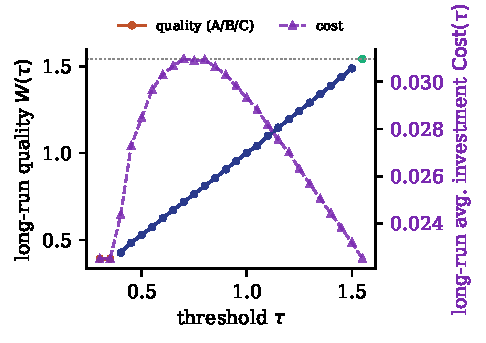
\includegraphics[width=0.55\linewidth]{figures/fig_costwelfare.pdf}
\caption{Long-run quality $W(\tau)$ (left axis) against long-run average investment $\mathrm{Cost}(\tau)$ (right axis), $\rho=0.30$ fixed. Cost is hump-shaped within Case (b), returning to the drift-offsetting rate $c_\delta$ at both boundaries while quality is monotonically higher at the upper one.}
\label{fig:costwelfare}
\end{figure}

\subsection{Calibrating to Real Audit Disclosures: Further Detail}

NYC Local Law 144 has required annual bias audits since July 2023, so real compliance-disclosure data now exists. We do not have, and as we discuss in Section~\ref{sec:discussion}, no one yet has, a firm-level panel suitable for testing the kink or cycling predictions directly, but the disclosures that do exist can ground the plausibility of our parameterization rather than leave $\tau = 0.80$ and the qualitative shape of the trajectories purely stylized.

Two independent field studies give the relevant statistics, and they are in some tension with each other, which we note rather than paper over. Wright et al.~\cite{wright2024null} collected 386 impact-ratio measurements from the disclosures posted by a self-selected subset of 391 covered NYC employers in late 2023 and found 96\% exceeded $0.8$, with 20\% of values missing (concentrated in smaller demographic groups). Gerchick et al.~\cite{gerchick2025auditing} extended data collection from July 2023 through November 2024 and report a substantially larger below-threshold share: 53\% of audits contained at least one impact ratio below $0.8$, and 23\% of group-level results fell below $0.8$ (rising to a bound of 28\% under conservative treatment of missing data). Differences in sampling window, unit of analysis (report-level versus group-level), and treatment of missing data likely explain most of the gap between the two studies' below-threshold shares; we do not have a way to adjudicate between them with currently available data. Gerchick et al. additionally report that reported ratios cluster tightly at or just above $1.0$ with a thin left tail; this is clustering at demographic parity, a full $0.2$ above $\tau=0.80$, not clustering at the legal threshold itself, so it speaks to firms' general performance level rather than directly to our model's predicted bunching around $\tau$. What the combined evidence does support is qualitatively looser: a nontrivial share of employers (Gerchick et al.'s 23--28\%) report ratios below $0.8$, which is inconsistent with a population made up entirely of Case A firms (which, once certified, remain at or above $\tau$ in steady state) and more consistent with a population that includes Case B firms cycling around $\tau$, caught below it depending on the audit date. This gives an empirical anchor for treating $\tau = 0.80$ as the economically relevant threshold in our simulations, rather than an arbitrary modeling choice.

We stop short of a stronger claim. Gerchick et al. identify only 13 audit reports with results in both 2023 and 2024, the entire currently-documented same-employer repeat-disclosure set, and document that employers frequently overwrite prior-year disclosures at the same URL rather than preserving them, that no tool-version identifiers are recorded (so a change in reported ratio cannot be attributed to drift versus re-audit of a modified system), and that only a small, self-selected fraction of covered employers post any audit report at all. These are exactly the obstacles that make a staggered-adoption or event-study test of Theorem~\ref{prop:recurring}'s predictions infeasible with currently available data, as flagged in Section~\ref{sec:discussion}'s limitations; a calibration exercise anchored on cross-sectional distributions is what the current data supports, and it is what we report here.

\section{Full Derivation of the Closed-Form Steady State}
\label{app:derivation}

This appendix gives the complete algebra behind the closed-form steady state $q^*(p)$ used in Section~\ref{sec:sim-recurring}, under the baseline calibration $f(c) = a\sqrt{c}$, $L(q) = b/(q+1)$. Every step follows directly from Assumption~\ref{as:steadystate}'s defining equation~\eqref{eq:steadystate}; nothing here is new relative to the main text, it is only spelled out at a finer grain.

\paragraph{Step 1: the drift-offsetting investment $c_\delta$.} By definition, $c_\delta$ is the investment level satisfying $f(c_\delta) = \delta$. With $f(c) = a\sqrt{c}$,
\[
a\sqrt{c_\delta} = \delta \quad\Longrightarrow\quad \sqrt{c_\delta} = \frac{\delta}{a} \quad\Longrightarrow\quad c_\delta = \left(\frac{\delta}{a}\right)^2.
\]

\paragraph{Step 2: the marginal return $f'(c_\delta)$.} Differentiating $f(c)=a\sqrt{c}$ gives $f'(c) = a/(2\sqrt{c})$. Evaluating at $c=c_\delta$ and substituting $\sqrt{c_\delta}=\delta/a$ from Step 1,
\[
f'(c_\delta) = \frac{a}{2\sqrt{c_\delta}} = \frac{a}{2\,(\delta/a)} = \frac{a^2}{2\delta}.
\]

\paragraph{Step 3: the marginal harm $|L'(q)|$.} Differentiating $L(q) = b/(q+1)$ gives $L'(q) = -b/(q+1)^2$, so
\[
|L'(q)| = \frac{b}{(q+1)^2}.
\]

\paragraph{Step 4: substituting into the steady-state equation.} Assumption~\ref{as:steadystate}'s defining equation~\eqref{eq:steadystate}, $\beta\,p\,|L'(q^*(p))|\,f'(c_\delta) = 1$, becomes, using Steps 2 and 3,
\[
\beta\, p\, \frac{b}{(q^*(p)+1)^2}\, \frac{a^2}{2\delta} = 1.
\]
Rearranging to isolate $(q^*(p)+1)^2$,
\[
(q^*(p)+1)^2 = \frac{p\,\beta\,a^2\,b}{2\delta}.
\]
Since $q^*(p)+1 > 0$ on the domain where Assumption~\ref{as:L} holds ($q > -1$, per Assumption~\ref{as:L}'s remark on the calibration used here), the positive square root is the economically meaningful one:
\[
q^*(p) = \sqrt{\frac{p\,\beta\,a^2\,b}{2\delta}} - 1,
\]
which is the closed form used in Section~\ref{sec:sim-recurring} and evaluated there at $p=p_H=1.0$ and $p=p_L=\rho\,p_H$ for the reported figures.


\end{document}
